\pdfoutput=1
\pdfcompresslevel=9
\pdfinfo
{
    /Author (Autor)
    /Title (Tytul)
    /Subject (Tematyka)
    /Keywords (Slowa kluczowe)
}
%\documentclass[a4paper,polish,onecolumn,oneside,floatssmall,11pt,titleauthor,wide,openright]{mwrep}
%\usepackage[scale={0.7,0.8},paper=a4paper,twoside]{geometry}
\documentclass[a4paper,onecolumn,oneside,11pt,wide,floatssmall]{mwrep}
% \usepackage{polish}
\usepackage{amsmath}
\usepackage{amsfonts}
\usepackage{amssymb}
\usepackage{amsthm}
\usepackage{bookman}

\usepackage{geometry}
\usepackage[utf8x]{inputenc}
\usepackage[T1]{fontenc}
% \usepackage{t1enc}
% \usepackage[pdftex, bookmarks]{hyperref}
\usepackage[pdftex, bookmarks=false]{hyperref}
\def\url#1{{ \tt #1}}

\usepackage{listings}
\usepackage{float}

% marginesy
\textwidth\paperwidth
\advance\textwidth -55mm
\oddsidemargin-0.9in
\advance\oddsidemargin 33mm
\evensidemargin-0.9in
\advance\evensidemargin 33mm
\topmargin -1in
\advance\topmargin 25mm
\setlength\textheight{48\baselineskip}
\addtolength\textheight{\topskip}
\marginparwidth15mm

\clubpenalty=10000 % to kara za sierotki
\widowpenalty=10000 % nie pozostawia wdów
\brokenpenalty=10000 % nie dzieli wyrazów pomiędzy stronami
\sloppy

\tolerance4500
\pretolerance250
\hfuzz=1.5pt
\hbadness1450

% ŻYWA PAGINA
\renewcommand{\chaptermark}[1]{\markboth{\scshape\small\bfseries \
#1}{\small\bfseries \ #1}}
\renewcommand{\sectionmark}[1]{\markboth{\scshape\small\bfseries\thesection.\
#1}{\small\bfseries\thesection.\ #1}}
\newcommand{\headrulewidth}{0.5pt}
\newcommand{\footrulewidth}{0.pt}
\pagestyle{uheadings}

\usepackage[pdftex]{color,graphicx}
\usepackage[polish]{babel}

% \textheight232mm
% \setlength{\textwidth}{\textwidth}
% \setlength{\oddsidemargin}{\evensidemargin}
% \setlength{\evensidemargin}{0.3cm}
\usepackage[sort, compress]{cite}

%\usepackage{multibib}
%\newcites{bk,st,doc,web}{Książki i~artykuły,Standardy i~zalecenia,Dokumentacja produktów,Publikacje i~serwisy internetowe}

\theoremstyle{definition}
\newtheorem{defn}{Definicja}[section]
\newtheorem{conj}{Teza}[section]
\newtheorem{conjmain}{Teza}
\newtheorem{exmp}{Przykład}[section]

\theoremstyle{plain}% default
\newtheorem{thm}{Twierdzenie}[section]
\newtheorem{lem}[thm]{Lemat}
\newtheorem{prop}[thm]{Hipoteza}
\newtheorem*{cor}{Wniosek}

\theoremstyle{remark}
\newtheorem*{rem}{Uwaga}
\newtheorem*{note}{Uwaga}
\newtheorem{case}{Przypadek}

\definecolor{ListingBackground}{rgb}{0.95,0.95,0.95}

\begin{document}

% kody źródłowe wplatane w tekst
\lstdefinestyle{incode}
{
basicstyle={\footnotesize},
keywordstyle={\bf\footnotesize\color{blue}},
commentstyle={\em\footnotesize\color{magenta}},
numbers=left,
stepnumber=5,
firstnumber=1,
numberfirstline=true,
numberblanklines=true,
numberstyle={\sf\tiny},
numbersep=10pt,
tabsize=2,
xleftmargin=17pt,
framexleftmargin=3pt,
framexbottommargin=2pt,
framextopmargin=2pt,
framexrightmargin=0pt,
showstringspaces=true,
backgroundcolor={\color{ListingBackground}},
extendedchars=true,
% title=\lstname,
captionpos=b,
% abovecaptionskip=1pt,
% belowcaptionskip=1pt,
frame=tb,
framerule=0pt,
}

% kody źródłowe z podpisem
\lstdefinestyle{outcode}
{
basicstyle={\footnotesize},
keywordstyle={\bf\footnotesize\color{blue}},
commentstyle={\em\footnotesize\color{magenta}},
numbers=left,
stepnumber=5,
firstnumber=1,
numberfirstline=true,
numberblanklines=true,
numberstyle={\sf\tiny},
numbersep=10pt,
tabsize=2,
xleftmargin=17pt,
framexleftmargin=3pt,
framexbottommargin=2pt,
framextopmargin=2pt,
framexrightmargin=0pt,
showstringspaces=true,
backgroundcolor={\color{ListingBackground}},
extendedchars=true,
% title=\lstname,
captionpos=b,
% abovecaptionskip=1pt,
% belowcaptionskip=1pt,
frame=tb,
framerule=0.1pt,
}

\renewcommand*\lstlistingname{Wydruk}
\renewcommand*\lstlistlistingname{Spis wydruków}

\pagenumbering{roman}
\renewcommand{\baselinestretch}{1.0}
\raggedbottom

\begin{titlepage}
    % Strona tytułowa
    \vbox to\textheight{\hyphenpenalty=10000
    \begin{center}
	\begin{tabular}{p{107mm} p{9cm}}
	    \begin{minipage}{9cm}
	      \begin{center}
	      Politechnika Warszawska \\
	      Wydział Elektroniki i~Technik Informacyjnych \\
	      Instytut Informatyki
	      \end{center}
	    \end{minipage}
	    &
	    \begin{minipage}{8cm}
	    \begin{flushleft}
	     \footnotesize
	      Rok akademicki 200X/200Y
	    \vspace*{2.75\baselineskip}
	    \end{flushleft}
	    \end{minipage} \\
	\end{tabular}
	\vspace*{3.75\baselineskip}
	\par\vspace{\smallskipamount}
	\vspace*{2\baselineskip}{\LARGE Praca dyplomowa magisterska\par}
	\vspace{3\baselineskip}{\LARGE\strut Imię i Nazwisko\par}
	\vspace*{2\baselineskip}{\huge\bfseries Tytuł pracy\par}

	\vspace*{7\baselineskip}
	\hfill\mbox{}\par\vspace*{\baselineskip}\noindent
	\begin{tabular}[b]{@{}p{3cm}@{\ }l@{}}
	    {\large\hfill } & {\large }
	\end{tabular}
	\hfill
	\begin{tabular}[b]{@{}l@{}}
	Opiekun pracy: \\[\smallskipamount]
	{\large Tytuł Imię i Nazwisko}
	\end{tabular}\par
	\vspace*{4\baselineskip}
    \begin{tabular}{p{\textwidth}}
    \begin{flushleft}
	\begin{minipage}{7cm}
	Ocena \dotfill
	\par\vspace{1.6\baselineskip}
	\dotfill
	\par\noindent
	\centerline{\footnotesize Podpis Przewodniczącego} \par
	\centerline{\footnotesize Komisji Egzaminu Dyplomowego}\par
	\end{minipage}
    \end{flushleft}
    \end{tabular}
    \end{center}}

    % Życiorys
    \newpage\thispagestyle{empty}
    \begin{tabular}{p{5cm} p{12cm}}
    \begin{minipage}{5cm}
    \center
    
\includegraphics[height=6.5cm,width=4.5cm]{../img/foto.jpg}
    \end{minipage}
    &
    \begin{minipage}{12cm}
    \begin{flushleft}
    \par\noindent\vspace{1\baselineskip}
    \begin{tabular}[h]{l l}
    {\normalsize\it Specjalność:} & Informatyka -- \\
    & Inżynieria oprogramowania \\
    & i~systemy informacyjne
    \end{tabular}
    \par\noindent\vspace{1\baselineskip}
    \begin{tabular}[h]{l l}
    {\normalsize\it Data urodzenia:} & {\normalsize 1 stycznia 1980~r.}
    \end{tabular}
    \par\noindent\vspace{1\baselineskip}
    \begin{tabular}[h]{l l}
    {\normalsize\it Data rozpoczęcia studiów:} & {\normalsize 1 października 2002 r.}
    \end{tabular}
    \par\noindent\vspace{1\baselineskip}
    \end{flushleft}
    \end{minipage}
    \end{tabular}
    \vspace*{1\baselineskip}
    \begin{center}
	{\large\bfseries Życiorys}\par\bigskip
    \end{center}

    \indent
    Nazywam się  \ldots.
    \par
    \vspace{2\baselineskip}
    \hfill\parbox{15em}{{\small\dotfill}\\[-.3ex]
    \centerline{\footnotesize podpis studenta}}\par
    \vspace{3\baselineskip}
    \begin{center}
 	{\large\bfseries Egzamin dyplomowy} \par\bigskip\bigskip
    \end{center}
    \par\noindent\vspace{1.5\baselineskip}
    Złożył egzamin dyplomowy w dn. \dotfill
    \par\noindent\vspace{1.5\baselineskip}
    Z wynikiem \dotfill
    \par\noindent\vspace{1.5\baselineskip}
    Ogólny wynik studiów \dotfill
    \par\noindent\vspace{1.5\baselineskip}
    Dodatkowe wnioski i uwagi Komisji \dotfill
    \par\noindent\vspace{1.5\baselineskip}
    \dotfill

    % Streszczenie
    \newpage\thispagestyle{empty}
    \vspace*{2\baselineskip}
    \begin{center}
	{\large\bfseries Streszczenie}\par\bigskip
    \end{center}

    {\itshape
    Praca ta prezentuje \ldots}
    \vspace*{1\baselineskip}

    \noindent{\bf Słowa kluczowe}: {\itshape słowa kluczowe.}
    \par
    \vspace{4\baselineskip}
    \begin{center}
	{\large\bfseries Abstract}\par\bigskip
    \end{center}
    \noindent{\bf Title}: {\itshape Thesis title.}\par
    \vspace*{1\baselineskip}
    {\itshape
    This thesis describes \ldots}
    \vspace*{1\baselineskip}

    \noindent{\bf Key words}: {\itshape key words.}

\end{titlepage}

% ex: set tabstop=4 shiftwidth=4 softtabstop=4 noexpandtab fileformat=unix filetype=tex spelllang=pl,en spell:


\tableofcontents
% \addcontentsline{toc}{chapter}{{Przedmowa1}{vii}}{vii}

% \chapter*{Spis tablic, rysunków i~wydruków}
% \listoftables
% \listoffigures
% \lstlistoflistings

%\setlength{\baselineskip}{7mm}
\newpage
\pagenumbering{arabic}
\setcounter{page}{1}

% \chapter{Wprowadzenie}

Szblon ten jest propozycją składu pracy dyplomowej inżynierskiej lub
magisterskiej. Poniżej znajdują się przykłady pozwalające na
szybkie zapoznanie się z podstawowymi elementami dokumentu takimi jak
tablice, rysunki, wyliczenia itp.

Przed oddaniem tego dokumentu prawidłowo wypełnić jego początkowe strony
tj.:
\begin{itemize}
\item stronę tytułową: rocznik, typ (magisterska/inżynierska),
imię i~nazwisko autora, tytuł, imię i~ nazwisko promotora pracy,
\item życiorys: data urodzenia, datę rozpoczęcia studiów, zdjęcie i~
życiorys autora,
\item streszczenie oraz słowa kluczowe w~języku polskim i~angielskim.
\end{itemize}

Szczegółowe opcje klasy {\tt mwrep}, którą wykorzystuje ten dokument,
opisane są w~dokumentacji.

\section[Tytuł w paginie][Tytuł w spisie treści]{Przykład pierwszy}

Pozostałe pliki (w głównej gałęzi katalogu 5015) reprezentują logikę struktury
PKCS~\#15 oraz certyfikaty (pliki 4545, 4546, 4547). Jej szczegółowy
opis zamieszczono w~\cite[130-140]{bk:ipki}. W~
tablicy \ref{tab:card} zebrano podstawowe dane o~wszystkich plikach.
Rozmiar niektórych plików może być różny dla innych danych wejściowych.
Dotyczy to w~szczególności certyfikatów.

Należy przyjąć, że aplikacja PKCS~\#15 w~karcie zajmuje do 6kB. W~karcie
{\it Cryptoflex 32K} pozsostaje więc około 26 kB możliwych do wykorzystania
przez inne aplikacje. W~szczególności mogą to być kolejne aplikacje PKCS~\#15
o~innym profilu zastosowań.

\begin{table}
\centering
\caption{Wykaz plików karty {\it Cryptoflex 32K} z~aplikacją PKCS~\#15}
\label{tab:card}
\begin{minipage}{.9\textwidth}
\setlength{\baselineskip}{2mm}
\centering
\begin{tabular}{c|c|c|c}
FID\footnote{ang. {\em file identifier} -- identyfikator pliku} & Rozmiar\footnote{rozmiar plików zawierających certyfikaty może być inny (w zależności od umieszczonego certyfikatu)} & Rodzaj pliku & Podstawowe prawa\\
 & (w bajtach) & & dostępu\footnote{stosowane oznaczenia: R~(ang. {\em read}) -- odczyt, U~(ang. {\em update}) -- zmiana, C~-- operacje kryptograficzne, NEV (ang. {\em never}) -- nigdy, CHV1 (ang. {\em cardholder verification}) -- kod uwierzytelniający użytkownika, ALW (ang. {\em always}) -- zawsze, AUT (ang. {\em authenticate}) -- uwierzytelnienie z~użyciem klucza}\\ \hline
3F00		    & --		   & DF\footnote{ang. {\em dedicated file} -- plik dedykoway, katalog}	& -- \\ \hline
0011		    & 27		   & EF\footnote{ang. {\em elementary file} -- plik elementarny}	& R: NEV, U: AUT \\ \hline
0002		    & 8			   & EF, TR\footnote{ang. {\em transparent} -- struktura transparentna, przeźroczysta} & R: ALW, U: NEV \\ \hline
5015		    & --		   & DF		    & -- \\ \hline
4401\footnote{identyfikatory podano bez pełnych ścieżek, zobacz rysunek \ref{ppkcs15fs}}	    & 255		   & EF, TR		    & R: ALW, U: AUT \\ \hline
4402		    & 255		   & EF, TR		    & R: ALW, U: AUT \\ \hline
5031		    & 255		   & EF, TR		    & R: ALW, U: AUT \\ \hline
5032		    & 33		   & EF, TR		    & R: ALW, U: AUT \\ \hline
4545		    & 849		   & EF, TR		    & R: ALW, U: AUT \\ \hline
4546		    & 847		   & EF, TR		    & R: ALW, U: AUT \\ \hline
4547		    & 849		   & EF, TR		    & R: ALW, U: AUT \\ \hline
4946		    & 127		   & EF, TR		    & R: ALW, U: AUT \\ \hline
4B01, 4B02	    & --		   & DF		    & -- \\ \hline
0000		    & 16		   & EF, CHV\footnote{ang. {\em cardholder verification} -- kody służące do uwierzytelnienia użytkownika} & R: NEV, U: CHV1 | AUT \\ \hline
3045, 3047	    & --		   & DF		    & -- \\ \hline
0012		    & 326		   & EF, PRVK\footnote{ang. {\em private key} -- klucz prywatny} & R: NEV, U: AUT, C: CHV1 \\ \hline
1012		    & 330		   & EF, PUBK\footnote{ang. {\em public key} -- klucz publiczny} & R: ALW, U: AUT, C: ALW \\ \hline
2F00		    & 127		   & EF, TR		    & R: ALW, U: AUT \\
\end{tabular}
\end{minipage}
\end{table}

\subsubsection{Założenia}
Dany jest zbiór pewnych maszyn. Każda z~nich charakteryzuje się pewnym
typem i~lokalizacją. Maszyny złożone są z~pewnych modułów.

Każda z~maszyn raportuje do systemu centralnego zdarzenia jakie na niej
zachodzą. Należą one do jednej z~kategorii:
\begin{itemize}
\item normalne zdarzenie
\item błąd -- zdarzenie to zawiera opis zgłaszanego błędu (moduł);
wyróżniamy błędy krytyczne (maszyna nie działa) i~ostrzeżenia (np. brakuje
zasobów dla pewnego modułu)
\item interwencja -- o~kategorii lokalnej (np. maszyna sama się naprawiła)
lub zdalnej (wymagana interwencja człowieka)
\end{itemize}

Na maszynach zachodzą pewne transakcje, których przebieg raportowany jest w~
postaci normalnych zdarzeń (chyba, że w~trakcie pojawi się błąd).

Zdarzenia przechowywane są w~bazie danych. Jest to jedna tabela, w~której
zapisane są dane określające maszynę, data i~czas zdarzenia oraz jego opis.

\subsection{Przykład drugi}

Przykładowa struktura aplikacji zgodnej z~PKCS~\#15 została zaprezentowana
na rysunku \ref{ppkcs15fs}.
Kolejne elementy systemu plików odzwierciedlają instancje obiektów z~danymi
zdefiniowanymi w~PKCS~\#15. Ich szczegółowa budowa, określona z~użyciem
notacji ASN.1 (ang. {\em abstract syntax notation number 1})
przedstawiona jest w~samej normie.

\begin{figure}[htb]
    \begin{center}
	\includegraphics[angle=-90,scale=.6]{img/pkcs15fs.pdf}
	\caption{Przykładowa struktura aplikacji PKCS~\#15}
	\label{ppkcs15fs}
    \end{center}
\end{figure}

\begin{thm}
\label{thm}
Niech $x_1, x_2, x_3, \ldots$ będą dowolnymi zmiennymi o wartościach
należących do zbiorów $X_1, X_2, X_3, \ldots$.
\end{thm}

\begin{note}
Zdanie jest spełnione wyłącznie w dziedzinie $D_1$.
\end{note}

\begin{proof}[Dowód Twierdzenia \ref{thm}.]
Załóżmy, że twierdzenie \ref{thm} nie jest prawdziwe. Wtedy zachodzi:
\begin{equation}
G(t)=L\gamma!\,t^{-\gamma}+t^{-\delta}\eta(t) \qedhere
\end{equation}
\end{proof}

\section{Przykład trzeci}

W~ostatnim dziesięcioleciu, wraz z~silnym rozwojem aplikacji i~urządzeń
wykorzystujących algorytmy kryptograficzne, pojawiło się szereg problemów
związanych z~uniwersalnością zapisu danych wykorzystywanych podczas tych
operacji. Jedna z~amerykańskich firm, będąca liderem na rynku biznesowych
zastosowań kryptografii, postanowiła opracować własne formuły zapisu
informacji kryptograficznych. Brak dyskusji nad proponowanymi zaleceniami
(w przeciwieństwie do głosowania nad normami ISO/IEC) pozwolił na szybkie ogłoszenie
początkowych wersji dokumentów oraz ich wdrożenie. Pomysł przyjął się i~
dzięki temu powstały normy przemysłowe dotyczące kryptografii.

Firma {\bf RSA Data Security, Inc.}, bo o~niej mowa, zaproponowała szereg zaleceń
związanych z~interfejsem dla kryptografii z~kluczem publicznym. Znane są one pod
ogólną nazwą PKCS (ang. {\em Public Key Cryptography Standards}).
Wnioskując jedynie po ogólnym tytule można odnieść wrażenie, że zalecenia
objęły jedynie algorytmy asymetryczne (w których występuje para kluczy -
jawny, zwany publicznym oraz tajny, zwany prywatnym). Twórcy poruszyli
również tematykę związaną z~szerokim zastosowaniem tych algorytmów, dzięki
czemu zalecenia zawierają praktycznie wszystkie najważniejsze i~
najaktualniejsze informacje dotyczące praktycznych zastosowań kryptografii.

Lista dokumentów z~serii PKCS jest następująca:
\begin{itemize}
    \item PKCS \#1: {\em RSA Cryptography Standard} -- zawiera opis
    algorytmu RSA zarówno w~odniesieniu do podpisu cyfrowego jak i~
    kopert cyfrowych\footnote{dokumenty o~identyfikatorach \#2 i~\#4
    zostały połączone w~\#1}
    \item PKCS \#3: {\em Diffie-Hellman Key Agreement Standard} -- opisuje
    sposób implementacji algorytmu uzgadniania kluczy metodą
    Diffiego-Hellmana
    \item PKCS \#5: {\em Password-Based Cryptography Standard} -- zawiera
    opis metody bezpiecznej wymiany kluczy prywatnych
    \item PKCS \#6: {\em Extended-Certificate Syntax Standard} --
    opisuje budowę certyfikatów klucza publicznego X.509
    \item PKCS \#7: {\em Cryptographic Message Syntax Standard} -- jest to
    abstrakcyjny opis danych, które podlegają operacjom kryptograficznym
    \item PKCS \#8: {\em Private-Key Information Syntax Standard} --
    zawiera abstrakcyjny opis dotyczący składowania kluczy prywatnych (w
    formie jawnej i~zaszyfrowanej) wraz z~zestawem atrybutów
    \item PKCS \#9: {\em Selected Attribute Types} -- zawiera definicję
    atrybutów związanych z~certyfikatami, podpisami cyfrowymi i~kluczami
    prywatnymi
    \item PKCS \#10: {\em Certification Request Syntax Standard} --
    opisuje format żądania certyfikacyjnego
    \item PKCS~\#11: {\em Cryptographic Token Interface Standard} --
    opisuje abstrakcyjny interfejs programisty dla różnych typów urządzeń
    kryptograficznych
    \item PKCS \#12: {\em Personal Information Exchange Syntax
    Standard} -- zawiera opis formatu zapisu danych kryptograficznych przez
    aplikacje
    \item PKCS \#13: {\em Elliptic Curve Cryptography Standard} -- zawiera
    opis algorytmów opartych na krzywych eliptycznych
    \item PKCS \#14: {\em Pseudo Random Number Generation} -- zawiera
    opis algorytmów związanych z~generacją liczb
    pseudolosowych\footnote{aktualnie dokument ten jest opracowywany}
    \item PKCS~\#15: {\em Cryptographic Token Information Format
    Standard} -- opisuje sposób zapisu danych w~żetonach kryptograficznych
    (takich jak karty procesorowe)
\end{itemize}

Wszystkie publikacje dostępne są pod adresem internetowym
\url{http://www.rsasecurity.com/rsalabs/}.

\section{Przykład czwarty}

{\it Xfig}\footnote{\url{http://www.xfig.org/}}
i~{\it Dia}\footnote{\url{http://www.gnome.org/projects/dia/},
\url{http://dia-installer.sourceforge.net/}}
to aplikacje wspomagające tworzenie rysunków w~grafice wektorowej.
Pierwsza z~nich przeznaczona jest głownie do tworzenia obrazów
z~prostych elementów takich jak linie, prostokąty, okręgi, łuki.
{\it Dia}, wzorowane na {\it Visio} firmy {\it Microsoft}, posiada
wiele bibliotek graficznych i~jest najbardziej pomocne do
tworzenia skomplikowanych diagramów np. w~UML. Obie aplikacje obsługują
szeroki wachlarz formatów plików graficznych, co pozwala na wykorzystanie
rysunków stworzonych z~ich pomocą w~wielu programach służących do edycji
lub składu dokumentów.

Rysunek \ref{fig:xfig} obrazuje program {\it Xfig} podczas pracy nad jednym
z~rysunków wykorzystanych w~publikacji~\cite{bk:ipki}.
\begin{figure}[htb]
    \begin{center}
    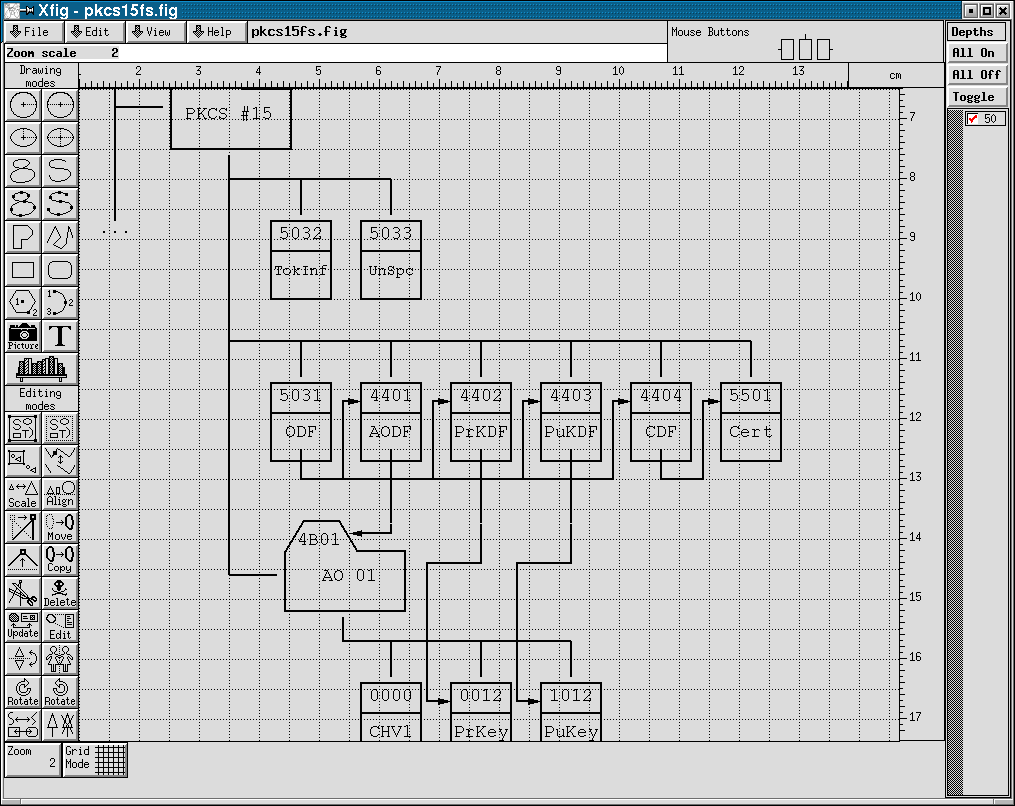
\includegraphics[angle=0,scale=.35]{img/xfig.png}
    \end{center}
    \caption{\em Xfig}
    \label{fig:xfig}
\end{figure}

\section{Przykład piąty}

Po utworzeniu pliku konfiguracyjnego można przystąpić do przygotowania
katalogów służących do przechowywania danych CA (zgodnie z~wcześniej
założonymi nazwami w~{\em openssl.cnf}). Tworzymy katalog {\em ca}, a~w nim
katalogi {\em certs}, {\em crl}, {\em private}, {\em newcerts} oraz pliki
{\em serial.txt} (z wpisem 01) i~{\em index.txt}. Plik {\em openssl.cnf} należy
umieścić na tym samym poziomie co katalog {\em ca}. Oczywiście możliwe jest
zupełnie inne zorganizowanie sposobu przechowywania danych w~CA, jednak
musi ono odpowiadać wcześniej przyjętym założeniom w pliku konfiguracyjnym.

Następnym krokiem przy tworzeniu CA jest wygenerowanie pary kluczy oraz
autocertyfikatu (w przypadku, gdy certyfikat dla centrum nie będzie
poświadczany przez inne centrum certyfikacji) dla centrum certyfikacji.

\begin{verbatim}
# generacja klucza prywatnego RSA o długości 4096 bitów
# do pliku cakey.pem (klucz w formie jawnej)
openssl genrsa -out ca/private/cakey.pem 4096 -config openssl.cnf

# utworzenie autocertyfikatu centrum (cacert.pem) o strukturze
# X.509 i formacie PEM dla klucza jawnego związanego z kluczem
# tajnym cakey.pem
openssl req -new -x509 -days 1825 -key ca/private/cakey.pem -out
    ca/cacert.pem -config openssl.cnf
\end{verbatim}

Po tych operacjach CA jest gotowe do pracy.

\section{Przykład szósty}

Oto przykładowy wydruk:
\begin{lstlisting}[language=Java,style=outcode,caption=Przykładowy wydruk]
import a.b.c;

// komentarz

/*
 * Komentarz...
 */
public class A
{
	int A;
	int B; // zmienna

	A()
	{
		A=1;
		/* to jest komentarz */
	}

	public void metodaA(int i)
	{
		for (int a=i; a<100; ++a)
		{
			short sw=(short)a;
			// ...
		}
	}
}
\end{lstlisting}

A oto wydruk wpleciony w tekst\dots
\begin{lstlisting}[language=C,style=incode]
/* ta funkcja oblicza a+b */
int sum(int a, int b)
{
	int suma=0;

	suma=a+b;

	return suma;
}
\end{lstlisting}
\dots i tekst za kodem.

% \lstinputlisting[language=Java,style=incode]{nazwa pliku}

% ex: set tabstop=4 shiftwidth=4 softtabstop=4 noexpandtab fileformat=unix filetype=tex spelllang=pl,en spell:

%%%% ROZDZIAŁ PIERWSZY %%%%%%%

\chapter{Analiza dziedziny} 
TODO opis tego co znajduje się w tym rozdziale, max 5 zdań


\section{Źródła informacji}

Analiza dziedziny powstała na wskutek agregacji i uporządkowania informacji 
z kilku źródeł. Posłużyłem się literaturą branżową, ustawą i informacjami z 
internetu jak również uzyskałem informację przeprowadzając rozmowy z 
pracownikami hotelu na różnym szczeblu. Miałem okazję rozmawiać z 
recepcjonistką oraz kierownikiem recepcji w dwóch różnych hotelach w 
Warszawie. Poniżej czytelnik znajdzie przefiltrowane, spójne wiadomości na
 temat branży hotelarskiej.


\section{Historia hotelarstwa} 

Ludzie zmieniali swoje miejsce od tysiącleci. Dlaczego? Powody były różne i 
przez tysiąclecia znacząco się nie zmieniły. Kiedyś wędrówki handlowe, a 
dziś wyjazdy biznesowe. Religijne wyprawy w miejsca kultu, podróże 
turystyczne do atrakcyjnych, bądź historycznych miejsc.     Historia 
hotelarstwa ma bogatą przeszłość i sięga aż II tysiąclecia p.n.e gdzie na 
terenach Bliskiego Wschodu znaleziono pierwsze ślady budownictwa 
nastawionego na gościnę podróżnych. Najstarsze domy zajezdne odnotowano 
wzdłuż szlaków handlowych w miejscach obfitujących w wodę pitną. W 
starożytnej Grecji i Rzymie budowano zajady w miejscach kultu religijnego, 
bądź miejsc odbywania się igrzysk. W czasach Średniowiecza gościny udzielano 
w klasztorach, początkowo nieodpłatnie, z czasem jednak gościna przyjęła 
formę rynkową. Edykt Karola Wielkiego nałożył na klasztory i kościoły 
obowiązek utrzymania hospicjów, gdzie podróżnym udzielano wyżywienia, 
kąpieli i opieki medycznej. Najgęstsza sieć hospicjów znajdowała się na 
terenie dzisiejszej Szwajcarii. Szwajcaria posiada najdłuższe tradycje 
hotelarskie i jest uważana za wzór hotelarstwa takiego jak znamy dzisiaj.


\section{Hotelarstwo i usługa hotelarska}

\subsection{Czym charakteryzuje się hotelarstwo?}

Hotelarstwo to forma działalności gospodarczej charakteryzująca się:
\begin{itemize} 
  \item szczególnym rodzajem gościnności - gościnność za odpłatnością,
  \item na działalność hotelu składają się różnego rodzaju usługi. Główne z 
  nich to usługi bytowe takie jak zapewnienie noclegu oraz wyżywienia,
  \item pobyt gości w hotelach jest z reguły określony w czasie i 
  krótkotrwały,
  \item zakres usług świadczonych przez hotelarzy powiększa się i integruje 
  z innymi działalnościami turystycznymi i rozrywkowymi.
\end{itemize}

\subsection{Definicja usługi hotelarskiej}

Czym jest usługa hotelarska? Na to pytanie odpowie treść ustawy o usługach 
turystycznych \cite{ust:tur}.

\begin{defn}{Usługa hotelarska}

krótkotrwałe, ogólnie dostępne wynajmowanie domów, mieszkań, pokoi, miejsc 
noclegowych, a także miejsc na ustawienie namiotów lub przyczep 
samochodowych oraz świadczenie, w obrębie obiektu, usług z tym związanych.

\end{defn}

Usługi hotelarskie zaspokajają więcej potrzeb niż może to wynikać z 
definicji, a są to: wypoczynek, pożywienie, nocleg, higiena, rekreacja, 
rozrywka, zapewnienie bezpieczeństwa, opieka nad zdrowiem, zapewnienie 
wygody, dobrej atmosfery pobytu i inne drobne usługi.

Pewne usługi są regulowane prawnie, poprzez przepisy dotyczące wymagań 
rodzajowych i kategoryzacyjnych. Jednakże abstrahując od przepisów można 
stwierdzić iż w interesie każdego hotelarza jest zapewnienie tak bogatej 
palety usług jak to możliwe, aby wyróżniać się na rynku i przyciągać gości. 
Spełnienie minimum wymaganego prawnie nie jest szczególnie atrakcyjne z 
punktu widzenia gościa. Więcej o usługach dowiemy się wkrótce.

\section{Klasyfikacja i kategoryzacja obiektów hotelarskich}
Klasyfikacja określa podział obiektów na rodzaje. Rodzaje obiektów różnią 
się miedzy sobą zakresem działalności.

Definicje obiektów określa Rozporządzenie Ministra Gospodarki i Pracy z dnia 
19 sierpnia 2004 roku, oto część z nich:

\begin{itemize}
  \item hotele - obiekty posiadające co najmniej 10 pokoi, w tym większość 
  miejsc w pokojach jedno- i dwuosobowych, świadczące szeroki zakres usług 
  związanych z pobytem klientów;
  \item motele - obiekty położone przy drogach, dysponujące parkingiem, 
  posiadające co najmniej 10 pokoi, w tym większość miejsc w pokojach jedno- 
  i dwuosobowych;
  \item pensjonaty - obiekty posiadające co najmniej 7 pokoi, świadczące dla 
  swoich klientów całodzienne wyżywienie;
  \item kempingi - obiekty strzeżone, umożliwiające nocleg w namiotach i 
  przyczepach samochodowych, domkach turystycznych lub innych obiektach 
  stałych, oraz przyrządzanie posiłków i parkowanie samochodów.
\end{itemize}

Rozporządzenie definiuje także domy wycieczkowe, schroniska młodzieżowe, 
schroniska i pola biwakowe. Wiele obiektów nie zostało zdefiniowanych, m.in. 
ośrodki wczasowe, kwatery prywatne, internaty, domy studenckie.


\subsection{Podział według kategorii} 
Obiekty hotelarskie można podzielić według różnych kategorii\cite[15-16]{
KlasKatZakHot}:

\begin{enumerate}
  \item według lokalizacji
    \begin{itemize}
      \item hotele miejskie
      \item obiekty wypoczynkowe, sportowe, kuracyjne
      \item motele - przy szlakach komunikacyjnych
    \end{itemize}
  \item według średniego pobytu gościa w obiekcie
    \begin{itemize}
      \item hotele i pensjonaty stale lub prawie stale czynne
      \item zakłady rezydenckie (minimum 10-15 dni)
      \item hotele dla przejezdnych (2-3 dni)
    \end{itemize}
  \item według zakresu świadczonych usług
    \begin{itemize}
      \item hotel pełny - pełny zakres usług
      \item hotel pensjonat - brak restauracji dla gości z zewnątrz, brak 
      napojów alkoholowych
      \item hotel garni - tylko wydawanie śniadań i prowadzenie bufetu
    \end{itemize}
  \item według okresu eksploatacji
    \begin{itemize}
      \item stałe
      \item sezonowe
    \end{itemize}
  \item według siedziby obiektu
    \begin{itemize}
      \item stałe
      \item ruchome - zakłady w okresie ferii, domki kempingowe, wagony 
      sypialne, samoloty
    \end{itemize}
  \item według dostępności
    \begin{itemize}
      \item otwarte - ogólnodostępne
      \item półotwarte - domy wczasowe, domy zdrojowe
      \item zamknięte - tylko dla określonych grup ludności - domy 
      akademickie, sanatoria
    \end{itemize}
\end{enumerate}

\subsection{Wymagania kategoryzacyjne}
Wymagania dla obiektów kategoryzowanych określa to samo rozporządzenie. 
Ustalono w nim następujące kategorie bazy noclegowej:

\begin{itemize}
  \item dla hoteli, moteli i pensjonatów - pięć kategorii oznaczonych 
  gwiazdkami,
  \item dla kempingów - cztery kategorie oznaczone gwiazdkami,
  \item dla domów wycieczkowych i schronisk młodzieżowych - trzy kategorie 
  oznaczane cyframi rzymskimi.
\end{itemize}

Kategoryzacja niesie ze sobą wymagania. Każda kategoria ma ściśle określone 
kryteria, które obiekt musi spełniać. Kryteria te określają minimalny poziom 
świadczonych usług. Wprowadzają też porządek do słownictwa i umożliwiają 
standaryzację obiektów. Poświęcę szczególną uwagę pięcio-gwiazdkowej 
kategoryzacji.

\subsection{Pięć gwiazdek}
Prawdopodobnie wszyscy znają ten podział, a przynajmniej wiedzą, że im 
więcej gwiazdek tym wyższy standard. Różne turystyczne oferty mamią nas 
gwiazdkami. Warto wiedzieć na co faktycznie możemy liczyć, ale czy na pewno 
nasze oczekiwania zostaną spełnione? Kategoryzacja istnieje w wielu krajach 
europejskich, ale jedna jest drugiej nie równa. Szczegółowość wymagań dla 
kategorii różni się pomiędzy krajami. Nie wszędzie jest to także regulowane 
prawnie. W Niemczech nie ma kategoryzacji, a kategorie obiektów są stosowane 
w sposób umowny przez wydawców przewodników i biura podróży. Warto mieć to 
na uwadze przy następnej podróży.

\section{Podział usług hotelarskich}   
Omówię podział usług hotelarskich, a następnie krótko je zcharakteryzuję na 
podstawie \cite[8-10]{OrgaDzialHot}.

Podstawowymi usługami świadczonymi przez hotel są usługi noclegowe i 
gastronomiczne. Wszystkie inne usługi są im podporządkowane.

Wszystko co wykracza poza usługi podstawowe można podzielić w następujący 
sposób:
  \begin{itemize}
    \item usługi uzupełniające
    \item usługi fakultatywne
    \item usługi towarzyszące
  \end{itemize}

\subsection{Usługi uzupełniające}
Usługi uzupełniające uzupełniają podstawowe usługi i są z nimi bezpośrednio 
związane. Gość jest zmuszony z nich korzystać w momencie gdy decyduje się na 
pobyt w hotelu. Przykładami usług uzupełniających są:

\begin{itemize}
  \item budzenie
  \item szatnia
  \item depozyt
  \item informacja turystyczna
\end{itemize}

Usługi uzupełniające są zazwyczaj bezpłatne, ponieważ są wliczone w cenę 
usług podstawowych.

\subsection{Usługi fakultatywne}
Kolejny rodzaj usług to usługi fakultatywne. Te usługi są już mniej 
powiązane z usługami podstawowymi. Usługi fakultatywne uatrakcyjniają pobyt 
gościom. Przykłady usług:

\begin{itemize}
  \item basen
  \item sauna
  \item tenis
  \item rozrywka
\end{itemize}

Podczas pobytu korzystanie z nich jest opcjonalne, ale zazwyczaj trzeba być 
gościem hotelu, żeby móc z nich skorzystać. To czy te usługi są płatne czy 
nie zależy od hotelu.  Jeśli są bezpłatne, stanowią zachętę dla gości (mimo 
tego, że mogą być wliczone w cenę).

\subsection{Usługi towarzyszące}
Usługi towarzyszące są całkowicie ortogonalne w stosunku do usług 
podstawowych. Oznacza to, że nie trzeba być hotelowym gościem, aby móc z 
nich skorzystać. Tak samo jak usługi fakultatywne, usługi towarzyszące są 
opcjonalne. Usługi towarzyszące to odrębny rodzaj działalności z lokalizacją 
przy hotelu. Przykładami usług towarzyszących są:

\begin{itemize}
  \item kiosk
  \item kwiaciarnia
  \item kasyno
  \item usługi handlowe
\end{itemize}

\subsection{Usługi obce}
Te usługi, które są świadczone bezpośrednio przez obsługę hotelową nazywa 
się usługami własnymi. Są jednak pewne usługi dodatkowe, których hotel nie 
może, bądź nie jest to opłacalne, świadczyć. Sprzedawanie usług dodatkowych 
korzystając z zewnętrznych firm pozwala hotelowi zwiększyć swoją \mbox{atrakcyjność.} Przykładem usług obcych mogą być wszelakiej maści usługi turystyczne, 
które organizuje zewnętrzne biuro turystyczne.

Usługi obce to także dostarczanie energii elektrycznej, wody i innych mediów.
 Tutaj hotel jest zdany na innych, ponieważ samemu nie może wszystkiego 
wytworzyć.

\subsection{Wymagania kategoryzacyjne, a usługi}
Część usług dodatkowych może być wymuszona poprzez wymagania kategoryzacyjne.
 Te usługi są \emph{obowiązkowe}. Reszta usług dodatkowych, świadczonych 
 przez hotel dla wygody gości i podniesienia prestiżu 
 hotelu, to usługi \emph{dobrowolne}.

\section{Istotne definicje}
Przedstawię definicję noclegu oraz doby hotelowej. Następnie przedstawię 
definicję klienta i agenta. Więcej o klientach dowiemy się w
 \ref{rodzaje-klientow}.

\subsection{Definicja noclegu}

\begin{defn}{Nocleg}

Usługa noclegowa dla jednej osoby w wymiarze jednej doby hotelowej tzw. 
osobodzień. Nocleg jest jednostką miary usługi noclegowej.

\end{defn} 

Nocleg wykorzystywany jest w miernikach usług hotelarskich:
\begin{itemize}
  \item nominalna liczba noclegów - ilość miejsc, które można wynająć w 
  danym okresie.
  \item wskaźnik frekwencji - stopień wykorzystania miejsc w procentach
\end{itemize}

\subsubsection{Wskaźnik RevPAR}
Podstawowym wskaźnikiem jest wskaźnik RevPAR\footnote{skrót: Revenue per 
available room}. RevPAR określa zrealizowane, 
dzienne obroty każdego wybudowanego pokoju. Liczony jest na podstawie
 ilorazu dochodów z pokojów do dostępnych pokojów. RevPAR uwzględnia tylko 
 dochód z wynajmu pokojów. Nie brane są pod uwagę inne źródła dochodu.

\begin{equation}
RevPAR = \frac{Rooms Revenue}{Rooms Available}
\end{equation}

Może być także oszacowany w następujący sposób:

\begin{equation}
RevPAR \approxeq Freq \cdot ADR
\end{equation}

\begin{description}
  \item[Freq] wskaźnik frekwencji. Procent okupowanych pokoi.
  \item[ADR]\footnote{ang. {\em Average Daily Rate} } średnia stawka(netto) 
  za pokój bez śniadania. ADR liczone jest jako iloraz przychodów netto ze 
  sprzedaży pokoi i ilości sprzedanych pokoi.

\end{description}

\subsection{Definicja doby hotelowej}
Doba hotelowa różni się od zwykłej doby.

\begin{defn}{Doba hotelowa} - trwa do godziny określonej jako godzina 
zakończenia doby 
hotelowej. Godzina zakończenia doby hotelowej jest ustalana przez hotel.
 Długość doby hotelowej dla gościa może być większa lub mniejsza 
od normalnej doby. Doba hotelowa została wprowadzona ze względu na 
organizację pracy hotelu, m.in. sprzątania pokojów.

\end{defn}

Załóżmy, że godzina zakończenia doby hotelowej to 12.00. Jeśli gość 
przyjechał o godzinie 10 to będzie mógł korzystać z pokoju do godziny 12 
następnego dnia, a więc więcej niż 24 godziny. Przyjeżdżając po godzinie 12 
będzie mógł korzystać z pokoju krócej. W obu przypadkach gość zapłacił tyle 
samo za pojedynczą dobę hotelową.


\subsection{Klient}

Klient, bądź gość również został zdefiniowany w ustawie\cite{ust:tur}:

\begin{defn}{Klient}
- osoba, która zamierza zawrzeć lub zawarła umowę o świadczenie usług 
turystycznych na swoją rzecz lub na rzecz innej osoby, a zawarcie tej umowy 
nie stanowi przedmiotu jej działalności gospodarczej, jak i osobę, na rzecz 
której umowa została zawarta, a także osobę, której przekazano prawo do 
korzystania z usług turystycznych objętych uprzednio zawartą umową.

\end{defn}

Definicja bazująca na ustawie jest dość skomplikowana, więc można spróbować 
prościej:

\begin{defn}{Klient}
- osoba, korzystająca z usług hotelarskich, w szczególności usługi noclegowej
.

\end{defn}

Klient oraz gość nie znaczą dokładnie tego samego, ponieważ jak wiemy, 
hotel świadczy usługi towarzyszące, których świadczeniobiorca nie musi być 
gościem hotelowym. Jednak nie wdając się w szczegóły, 
będziemy używać tych nazw wymiennie. Więcej o klientach dowiemy się w 
\ref{rodzaje-klientow}

\subsection{Agent}
Agent biura turystycznego pełni rolę pośrednika. Zazwyczaj biuro turystyczne 
wykupuje pewny pakiet noclegów w hotelu. Kupując hurtowo otrzymuje niższe 
ceny, niż zwykli klienci, a zatem może pozwolić sobie na ciekawszą ofertę. 
Oto definicja agenta\cite{ust:tur}:

\begin{defn}{Agent turystyczny}
przedsiębiorca, którego działalność polega na stałym pośredniczeniu w 
zawieraniu umów o świadczenie usług turystycznych na rzecz organizatorów 
turystyki posiadających zezwolenia w kraju lub na rzecz innych usługodawców 
posiadających siedzibę w kraju.
\end{defn}

\section{Organizacja w zakładzie hotelarskim}
Przyjrzymy się teraz organizacji w zakładzie hotelarskim. Organizacja w 
zakładzie hotelarskim zależy od typu zakładu hotelarskiego. 

Inaczej będzie wyglądać organizacja w małym pensjonacie, prowadzonym przez 
kilka osób (np. rodzinę), a inaczej wyglądać będzie organizacja dużego 
luksusowego hotelu nastawionego na klientów biznesowych. 

W pierwszym przypadku członkowie rodziny i kilku pracowników mają szeroki 
zakres obowiązków i oczekiwane jest wykonywanie działań, które aktualnie są 
potrzebne. Struktura organizacja będzie dość prosta i płaska.

W przypadku znacznie większego hotelu, który zatrudnia znaczącą liczbę 
pracowników i obsługuje kilkuset gości wymagana będzie bardziej rozbudowana 
struktura organizacyjna. Przyjrzymy się podobnemu przypadkowi z bliska i 
poznamy jak może wyglądać taka struktura. 

Zanim jednak do tego przejdziemy zapoznajmy się z definicją struktury.

\subsection{Definicja struktury}
Definicja na podstawie \cite{bk:def-struktury}:
\begin{defn}{Struktura} 
to instrument zarządzania organizacją. To uporządkowanie pozycji w 
organizacji według zasad podziału pracy, co wiąże się z określeniem 
specjalistycznych zadań, które muszą być wykonane, aby organizacja mogła 
funkcjonować i osiągać założone cele. To zgrupowanie ról organizacyjnych w 
większe całości, podsystemy: sekcje, wydziały, zakłady, piony - gdzie 
następuje obarczenie odpowiedzialnością za sprawną realizację zagregowanych 
zadań poszczególnych komórek organizacyjnych, a zwłaszcza kierowników tych 
podsystemów. To w końcu podział władzy i informacji w ramach organizacji, a 
więc uporządkowanie pionowego podziału pracy w ramach szczebli struktury(
poziomów jej hierarchii)
\end{defn}

\subsection{Struktura organizacyjna w średniej wielkości hotelu}
Pod lupę weźmiemy średniej wielkości hotel. Na tyle duży, że wymaga 
wprowadzenia struktury organizacyjnej, ale na tyle skomplikowanej, że można 
będzie ją przedstawić w prosty sposób.

\subsubsection{Przykład struktury organizacyjnej hotelu}
Przykładową strukturę organizacyjną przedstawia poniższy rysunek 
\ref{fig:struktura-hotelu}.

\begin{figure}[H]
  \begin{center}
  \fbox{
    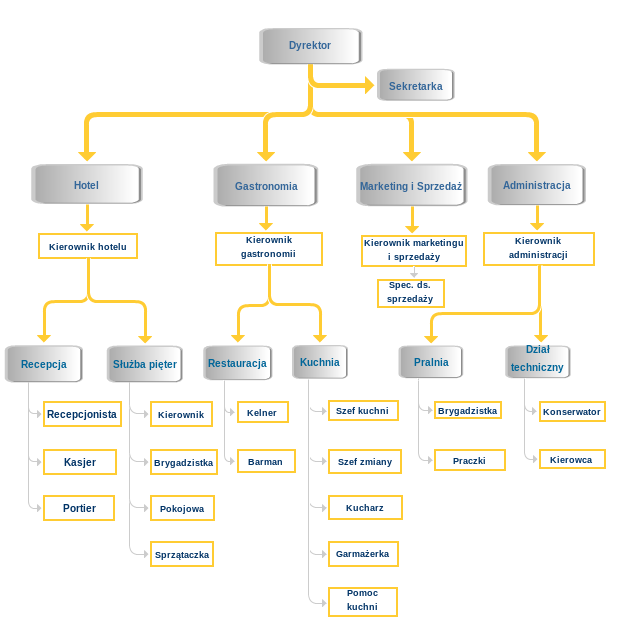
\includegraphics[width=\textwidth]{../img/struktura.png}
  }
  \end{center}
  \caption{Przykładowa struktura hotelu}
  \label{fig:struktura-hotelu}
\end{figure}

\subsubsection{Charakterystyka przykładowej struktury}
Na szczycie znajduje się dyrektor, ale bardziej interesujący jest dalszy 
podział. Struktura zawiera w sobie dwie struktury:
\begin{itemize}
  \item struktura produkcyjna - zaliczają się do niej wszystkie działy i 
  komórki, które w sposób bezpośredni związane są z \emph{produkcją}
  jednostki mieszkalnej gotowej do sprzedaży, sali konferencyjnej do 
  wynajmu, posiłku do wydania;
  \item struktura administracyjna - do której należą wszystkie działy, które
   nie są w strukturze produkcyjnej. Na rysunku pominąłem dział księgowy, 
   który jak najbardziej istnieje i zalicza się do struktury administracyjnej
   .
\end{itemize}

Struktura podzielona jest na 4 działy:
\begin{itemize}
  \item Dział Hotelarski - omówiony poniżej
  \item Dział Gastronomiczny - odpowiada za przygotowanie posiłków i napoi 
  do sprzedaży. Zapewnia gościom hotelowym wyżywienie w zakresie co najmniej 
  śniadania,
  \item Dział Marketingu i Sprzedaży - realizuje działania w efekcie, 
  których klient wybiera ten, a nie inny hotel,
  \item Dział Administracyjny - finanse, remonty, usługi wewnętrzne, 
  koordynacja działania przedsiębiorstwa
\end{itemize}

Działania tych działów muszą być koordynowane, tak aby każdy z nich 
efektywnie uczestniczył w zaspokajaniu potrzeb gości.

Za każdy dział odpowiedzialny jest kierownik, który odpowiada przed 
dyrektorem. Dyrektor nadzoruje i koordynuje działania kierowników.

\subsection{Dział Hotelarski}
W naszym przykładzie dział hotelarski składa się z:
\begin{itemize}
  \item węzła recepcyjnego - scharakteryzowanego poniżej,
  \item służba pięter - odpowiada za utrzymanie czystości w hotelu oraz za 
  przygotowanie jednostek mieszkalnych do sprzedaży oraz ciągów 
  komunikacyjnych do użytkowania.
\end{itemize}

Wymienione wyżej działy to tylko przykład, a prawdziwa struktura 
organizacyjna może być o wiele bardziej skomplikowana.

Przyjrzyjmy się bliżej węzłowi recepcyjnemu.

\subsection{Węzeł recepcyjny}
Recepcja pełni ważną rolę w strukturze organizacyjnej. Od strony gościa, 
można powiedzieć, że nawet najważniejszą. 
Recepcja obsługuje klienta od momentu przyjęcia rezerwacji, w ciągu pobytu, 
aż do zakończenia pobytu i opuszczenia przez gościa hotelu. Recepcja spełnia 
także funkcje marketingowe 
oraz sprzedażowe. Posiada także funkcje zakwaterowania i obsługi gościa 
podczas pobytu. Jako, że sam proces zakwaterowania jest bardzo krótki i trwa 
kilka, kilkanaście minut można powiedzieć, że najważniejszą i główną funkcją 
węzła recepcyjnego jest obsługa gościa w trakcie jego pobytu.

Recepcja pełni także funkcję sprzedażową, ponieważ klient, 
który przyjdzie wprost z ulicy chcąc wynająć pokój skieruje się recepcji. 
Jest to zatem  bardzo ważna komórka i jedna z pierwszych, z którą spotyka 
się gość podczas swojego pobytu. Oprócz tego pracownicy recepcji, mogą 
oferować płatne usługi, co także tłumaczy funkcję sprzedażową.

Potocznie mówi się, że pierwsze wrażenie jest najważniejsze. Recepcja jest 
dobrym tego przykładem. To od pracowników recepcji zależy, jakie będzie 
pierwsze wrażenie na kliencie. Od jakości obsługi podczas pobytu zależeć 
będzie czy pierwsze wrażenie zostanie utrzymane na dobrym poziomie oraz to 
czy klient opuści hotel szczęśliwy i będzie chciał wkrótce wrócić czy też nie
.


\subsubsection{Pracownicy recepcji}
W recepcji możemy spotkać \cite[47-51]{OrgaDzialHot}:

\begin{itemize}
  \item kierownika recepcji (front office manager) - odpowiada za sprawne 
  funkcjonowanie recepcji,
  \item recepcjonistę dysponenta - do jego zadań należy m.in przydzielanie 
  pokoi gościom na dany dzień na podstawie rezerwacji i pokoi zwalnianych,
  \item recepcjonista klucznik - m.in. zarządza kluczami, rozdziela 
  korespondencję, przyjmuje zlecenia na np. budzenie,
  \item recepcjonista ds. rezerwacji,
  \item recepcjonista kasjer - przyjmuje gotówkę, wymienia walutę,
  \item recepcjonista informator (consierge) - zajmuje się sprawami gości 
  hotelowych, np. zakup biletów na koncert.
\end{itemize}

\subsubsection{Obowiązki recepcji} 
Recepcja odpowiada za\cite[50]{OrgaDzialHot}:

\begin{itemize}
  \item przyjmowanie i realizacja zleceń na rezerwację miejsc noclegowych,
  \item przyjmowanie gości,
  \item wystawianie kart pobytu,
  \item prowadzenie ewidencji gości zgodnie z obowiązującymi zasadami,
  \item wydawanie kluczy do pokoi oraz prowadzenie właściwej ich ewidencji i 
  ich zabezpieczenie,
  \item organizowanie pomocy przy przyjazdach i wyjazdach ze szczególnym 
  uwzględnieniem opieki nad bagażem gości,
  \item udzielanie informacji gościom oraz realizowanie na ich rzecz 
  dodatkowych usług,
  \item sporządzanie codziennych grafików wykorzystania pokoi,
  \item sprawne działanie w przypadkach losowych,
  \item przyjmowanie reklamacji gości,
  \item opieka nad korespondencją,
  \item przyjmowanie mienia gości do depozytu.
\end{itemize}

\subsubsection{Zespoły recepcji}
W recepcji można wyróżnić następujące zespoły\cite[8-10]{hotel2:part1}:
\begin{enumerate}
  \item hall recepcyjny - część ogólnodostępna,
  \item lada recepcyjna,
  \item cześć wewnętrzna, usytuowana z reguły za ladą,
  \item służba parterowa.
\end{enumerate}

\section{Klasyfikacja hoteli raz jeszcze}
Wcześniej zapoznaliśmy się z klasyfikacją obiektów hotelarskich. Teraz 
chciałbym przedstawić prosty podział hoteli\footnote{obiektów hotelarskich 
rodzaju ,,hotel''}.

W pierwszym spojrzeniu na hotel, jego organizację, świadczone usługi i 
hotelowych gości można go zaklasyfikować do jednej z dwóch grup:

\begin{itemize}
  \item Hotel Turystyczny
  \item Hotel Biznesowy
\end{itemize}

Różnice będą widoczne w usługach, wystroju wewnętrznym i zewnętrznym, 
lokalizacji i nastawieniu na klienta.

Różnica będzie także w rocznym obłożeniu hoteli. Hotele turystyczne będą 
cieszyć się wysokim obłożeniem w sezonie turystycznym i zazwyczaj 
mniejszym poza okresem. Porównując obłożenia zauważymy, że hotele biznesowe 
charakteryzują się bardziej równomiernym obłożeniem w ciągu roku. 
Wyjątek stanowi okres konferencyjny, który rozpoczyna się na przełomie 
marca i kwietnia. Wówczas hotele biznesowe odnotowują zwiększone obłożenie,
 zwłaszcza te z dużą bazą konferencyjną.

Ciekawostką jest to, że pobyt w hotelu turystycznym będzie droższy w ciągu 
weekendu. Odwrotna sytuacja występuje w klasie biznesowej.

\section{Pomieszczenia hotelowe}
Hotel posiada liczne pomieszczenia. Tylko część z nich jest ogólnodostępna 
dla gości. Są to np. jednostki mieszkalne. Pomieszczenia można także 
podzielić na te, które dostępne są w określonych godzinach, a te które są 
dostępne całodobowo.

Niektóre pomieszczenia:
\begin{itemize}
\item hol,
\item recepcja,
\item jednostki mieszkalne,
\item sala restauracyjna,
\item sale konferencyjne,
\item magazyny,
\item zaplecze techniczne,
\item biura,
\item ciągi komunikacyjne,
\item winda,
\item korytarze.
\end{itemize}

Pomieszczeń hotelowych jest o wiele więcej, ale nie ma sensu ich wszystkich 
wymieniać. Przyjrzyjmy się bliżej jednemu pomieszczeniu.

\section{Pokoje}
Najbardziej znanym pomieszczeniem hotelowym są jednostki mieszkalne, czyli 
potocznie mówiąc pokoje hotelowe. Kontynuując opis naszego przykładowego 
hotelu, będziemy mogli przedstawić rodzaje pokojów w hotelu.

\subsection{Rodzaje pokojów}
Poniżej zostały wymienione rodzaje pokojów wraz z ich angielskimi nazwami.

Rodzaje pokoi hotelowych:
\begin{itemize}
  \item pokój jednoosobowy (ang. single room)
  \item pokój dwuosobowy (ang. double room)
  \item pokój trzyosobowy (ang. triple room)
  \item pokój z dostawką (ang. room with additional bed)
  \item pokój przystosowany do obsługi gości niepełnosprawnych (ang. room for 
  handicapped)
\end{itemize}

\section{Karta pobytu}
Karta pobytu to dokument, który otrzymuje gość po pomyślnym zakwaterowaniu. 
Karta pobytu zawiera najważniejsze informacje o dobie hotelowej, cieszy 
nocnej, warunkach bezpieczeństwa oraz usługach dodatkowych w hoteli i 
gastronomii. Może także zawierać szkic miasta z zaznaczonym hotelem.

Karta pobytu spełnia dwie funkcje:
\begin{itemize}
  \item{informacyjną}, przypomina gościom o podstawowych informacjach
  \item{zabezpieczającą} służy do identyfikacji gościa pobierającego klucz 
  lub podpisującego rachunek
\end{itemize}

\section{Rezerwacja}
Rezerwacja jest bardzo ważnym dokumentem w hotelarstwie. Jeszcze niedawno 
proces przyjmowania rezerwacji był jednym z częściej wykonywanych czynności 
przez recepcjonistę. Tam gdzie nie ma automatyzacji i możliwości dokonania 
rezerwacji przez internet nadal tak jest. Tam gdzie jest to proces manualny, 
tam też istnieje możliwość pomyłki. Prawidłowe dokonanie rezerwacji jest 
sprawą kluczową zarówno dla gościa jak i dla hotelu. Rezerwacja może bowiem 
stanowić źródło wielu dodatkowych informacji przydatnych przy organizacji 
usług hotelarskich i działań marketingowych.

W następnych podrozdziałach przyjrzymy się bliżej rezerwacji, gdyż jest to 
kluczowy element. Zapoznamy się w jaki sposób można jej dokonać, jakie są 
typy rezerwacji, jakie informacje zawiera i wiele dowiemy się o wielu innych 
rzeczach związanych z rezerwacją.

\subsection{Co oznacza rezerwacja?}
Rezerwacja, która jest niepotwierdzona od strony prawnej nie wiele znaczy. 
Między przyjęciem rezerwacji, a jej potwierdzeniem istnieje wiele wariantów, 
które mogą się wydarzyć w zależności od hotelu, ale z tym zapoznamy się 
później. 

Przyjęcie i potwierdzenie rezerwacji jest natomiast formą zawarcia umowy 
między gościem, a hotelem do realizacji podstawowej usługi hotelarskiej, 
czyli gościnności za odpłatnością. Aby zatem przyjąć rezerwację trzeba 
wiedzieć o obłożeniu hotelu, planowanych imprezach, planowanych remontach, 
tak aby móc zrealizować usługę w określonym terminie. Rezerwacja w ogólności 
jest dokonywana na typ pokoju, a nie konkretny pokój aczkolwiek może być 
inaczej. Wynika z tego, że trzeba wiedzieć jakie typy będą dostępne w 
określonym terminie.

\subsection{Sposoby przeprowadzania rezerwacji}
Sposobów dokonania rezerwacji jest kilka. Oto one:
\begin{itemize}
  \item dokonanie rezerwacji bezpośrednio w hotelu,
  \item dokonanie rezerwacji za pomocą faksu,
  \item dokonanie rezerwacji za pomocą internetu,
  \begin{itemize}
     \item bezpośrednio na stronie hotelu - uzupełniając formularz na 
     stronie hotelu
     \item pośrednio poprzez system klasy CRS \footnote{przykładowo 
     www.booking.com/index.pl.html} \ref{system-crs}
  \end{itemize}
  \item dokonanie rezerwacji poprzez rozmowę telefoniczną - podając dane 
  pracownikowi recepcji. Przez całą procedurę przeprowadzi nas pracownik w 
  recepcji.\footnote{W sieci hoteli Marriott wszystkie dane powtarzane są 
  dwa razy w celu sprawdzenia ich poprawności przez obie strony},
  \item dokonanie rezerwacji poprzez biuro usług pośredniczących - które  
  może korzystać z wcześniej wymienionych sposobów lub poprzez system klasy 
  CRS \ref{system-crs}. Istnieje jeszcze jedna możliwość, którą poznamy przy 
  okazji rezerwacji grupowych w \ref{rezerwacja-grupowa}
\end{itemize}

\subsection{Rodzaje rezerwacji}
W celu zabezpieczenia hotelu przed stratami z tytułu anulowanych rezerwacji, 
a tym samym niewykorzystanych pokoi wprowadzono trzy rodzaje rezerwacji:

\begin{itemize}
  \item wstępną,
  \item gwarantowaną,
  \item niegwarantowaną.
\end{itemize}

To czy wszystkie rodzaje rezerwacji są dostępne zależy od hotelu. 

\subsubsection{Rezerwacja wstępna}
Dokonujemy rezerwacji i otrzymujemy termin, do którego musimy potwierdzić 
rezerwację. W przypadku braku potwierdzenia rezerwacja zostaje anulowana. 
Żadna ze stron nie ponosi konsekwencji.

Jaki to będzie termin, zależeć będzie od hotelu. W przypadkach, gdzie 
głównie używana jest rezerwacja gwarantowana, może być tak, że terminem 
będzie godzina popołudniowa tego samego dnia, w którym dokonujemy rezerwację.
 Zatem ma to sens, jeśli już jesteśmy w drodze do hotelu i chcemy zrobić 
 rezerwację bez podawania numeru karty kredytowej.

\subsubsection{Rezerwacja gwarantowana}
Jest to typowy rodzaj rezerwacji. Aby dokonać rezerwacji potrzebna jest 
pewna forma gwarancji, a dokładnie pewne zabezpieczenie finansowe. Jest to 
najbezpieczniejszy rodzaj rezerwacji dla hotelu.

Forma zabezpieczenia może być różna. Może to być przedpłata w określonym 
terminie. Może to być także obciążenie karty kredytowej. Karta kredytowa to 
najczęściej spotykany sposób w przypadku dużych sieci hotelarskich. W naszym 
rodzimym przypadku spotkać się można z przedpłatą bankową.

Rezerwacja gwarantowana to sposób obrony hotelu przed stratami finansowymi. 
Jeśli gość zrezygnuje z rezerwacji to w zależności od terminu albo straci 
całe zabezpieczenie, albo część. Szczegóły zależą od zakładu hotelarskiego, 
ale zazwyczaj trzeba liczyć się z pewną karą.

Jeśli gość nie pojawi się planowanego dnia przyjazdu, to rezerwacja zostaje 
utrzymywana do dnia następnego, a gość zostaje obciążony kosztami pokoju za 
jedną noc, nie wliczając śniadania. Dalsza procedura zależy od hotelu, ale 
prawdopodobnie pracownik skontaktuje się z gościem, aby wyjaśnić zaistniałą 
sytuację. Koniec końców największy zysk jest z zadowolonego gościa 
hotelowego, a nie kar finansowych, które to zadowoleniu szkodzą.

Warto dodać, że metoda dokonania gwarancji nie ma związku z metodą płatności 
za pobyt.

\subsubsection{Rezerwacja niegwarantowana}
W odróżnieniu od rezerwacji gwarantowanej, dla tego typu rezerwacji nie ma 
konieczności zabezpieczenia w postaci depozytu. W przypadku nie 
wykorzystania rezerwacji w określonym terminie umowa przestaje obowiązywać, 
a jej rozwiązanie nie pociąga ze sobą żadnych skutków finansowych. Całe 
ryzyko ponosi zatem hotel. Łatwo sobie wyobrazić złe działania konkurencji, 
które mogą wykorzystać ten sposób rezerwacji.

\subsection{Pojedyncza i grupowa rezerwacja}
Kolejnym podziałem rezerwacji jest podział na rezerwację indywidualną oraz 
grupową. 

\subsubsection{Rezerwacja indywidualna}
Rezerwacja indywidualna to rezerwacja dla klienta indywidualnego, czyli taka 
jaką sami możemy zamówić w hotelu. Nie oznacza to jednak, że pobyt musimy 
spędzić samemu. Oznacza to, że rezerwacji dokonuje zwykła osoba. Dla tego 
typu rezerwacji ceny za pokój będą najwyższe.
Rezerwacja indywidualna może dotyczyć więcej niż jednego pokoju.

Zamiast samemu dokonywać rezerwacji możemy posłużyć się biurem pośrednictwa 
rezerwacji. Są to m.in biura turystyczne, biura linii lotniczych. Możliwe, 
że uda nam się wtedy zapłacić mniej, a dlaczego tak jest dowiemy się w 
\ref{biuro-turystyczne}

\subsubsection{Rezerwacja grupowa}
\label{rezerwacja-grupowa}
Rezerwacja grupowa to rezerwacja dla klienta grupowego. Rezerwacji grupowych 
dokonuje wiele różnych instytucji. Są to m.in biura turystyczne, korporacje, 
stowarzyszenia, agencje podróży. Za wszystkie formalności związane z 
dokonaniem rezerwacji odpowiedzialny będzie pośrednik wynajęty przez grupę, 
bądź organizatora pobytu dla grupy. Grupa oznacza wiele osób - rezerwacja 
grupowa dotyczyć będzie zatem wielu pokojów. 

Opłata za rezerwację grupową zależeć będzie od sposobu jej organizacji. W 
ogólnym przypadku pobyt opłacony będzie poprzez organizatora grupy. 
Natomiast to czy dodatkowe usługi\footnote{usługi towarzyszące i fakultatywne}
 również będą wliczone w cenę zależy od konkretnego przypadku. Istnieją trzy 
 możliwości:

\begin{itemize}
   \item organizator płaci za dodatkowe usługi,
   \item organizator nie płaci za dodatkowe usługi. Każdy członek grupy 
   płaci za korzystanie z usług,
   \item organizator płaci za dodatkowe usługi do pewnej kwoty. Nadwyżkę 
   opłaca członek grupy.
\end{itemize}

Ceny za pobyt będą atrakcyjniejsze w przypadku rezerwacji grupowych.

\subsubsection{Biuro turystyczne}
\label{biuro-turystyczne}
Biuro turystyczne jest jednym z podmiotów, które dokonują rezerwacji 
grupowych. Biura turystyczne posiadają także oferty dla klientów 
indywidualnych, w których koszta pobytu są niższe. Dlaczego tak jest?

Powody mogą być co najmniej dwa. Pierwsza możliwość jest taka, że biuro 
podróży nawiązuje z hotelem umowę, w której rezerwuje określoną liczbę 
pokoi wraz z określonymi usługami przy ustalonych warunkach cenowych - 
które będą korzystniejsze niż dla klienta indywidualnego. Najważniejszym dla 
biura jest termin, do którego musi powiadomić hotel o faktycznym 
wykorzystaniu miejsc. Jeśli w wyznaczonym terminie powiadomi hotel i 
zmniejszy ilość pokoi to obciążone zostanie tylko za wykorzystaną ilość, a 
reszta pokoi wróci do wolnej puli. Przy takiej umowie hotel zobowiązuje się, 
że określona ilość pokoi będzie dostępna i że nie będą one przedmiotem 
podobnej umowy z innym biurem turystycznym bądź inną instytucją.

Druga możliwość to tzw. \emph{allotment}. Biuro podróży wykupuje określoną 
ilość miejsc za bardzo atrakcyjną cenę. Umowa ta również określa, w jakim 
terminie biuro ma prawo zrezygnować z całości lub części zamówionych pokoi 
bez ponoszenia kosztów. Hotel nie może zawierać na te miejsca innych umów.

Tymi sposobami biuro podróży może pozwolić sobie zaoferować niższe ceny. 
Jeśli skorzystamy z oferty otrzymamy Voucher.

\begin{defn}{Voucher} 
to dokument indywidualny podobny do rezerwacji, który uprawnia beneficjenta 
do skorzystania z usługi.
\end{defn}

\subsection{Informacje na rezerwacji}
\label{chap1:info-na-rezerwacji}
Przy dokonywaniu rezerwacji możemy być pytani o wiele różnych informacji. 
Istnieje w miarę standardowa porcja informacji, którą zawsze trzeba podać. 
To ile szczegółowych informacji będziemy mogli podać zależeć będzie od 
\mbox{hotelu.} Bardzo szczegółową informacją są np. preferencje dotyczące 
rodzaju poduszki, bądź umiejscowienia pokoju blisko windy.

Podstawowe informacje, które podajemy przy dokonaniu rezerwacji to:

\begin{itemize}
  \item data przyjazdu,
  \item data wyjazdu,
  \item rodzaj pokoju,
  \item dane rezerwującego (klienta)
  \begin{itemize}
    \item tytuł,
    \item imię,
    \item nazwisko, 
    \item adres, 
    \item dane kontaktowe
  \end{itemize} 
  \item dane dla kogo jest rezerwacja
  \begin{itemize}
    \item tytuł,
    \item imię
    \item nazwisko
    \item osoby dodatkowe
  \end{itemize}
  \item metodę płatności
\end{itemize}

Niektóre z dodatkowych informacji, o które pytać będą hotele o wysokim 
standardzie:

\begin{itemize}
  \item czy pokój dla palących czy niepalących,
  \item umiejscowienie pokoju,
  \begin{itemize}
    \item niskie piętro,
    \item wysokie piętro,
    \item blisko windy,
  \end{itemize}
  \item widok,
  \item rodzaj poduszki,
  \item ile osób dorosłych,
  \item ile dzieci,
  \item informacje dodatkowe dla recepcji - specjalne życzenia bądź uwagi,
  \item preferencje żywieniowe.
\end{itemize}


\subsubsection{Potwierdzenie rezerwacji}
Potwierdzenie rezerwacji potwierdza dokonanie rezerwacji i tym samym jest 
zawiązaniem umowy między gościem, a hotelem. Potwierdzenie rezerwacji może 
być przekazane drogą elektroniczną bądź tradycyjną. Potwierdzenie rezerwacji 
pozwala na sprawdzenie poprawności danych. Potwierdzenie rezerwacji stwarza 
możliwość reklamy innych usług zakładu hotelarskiego. 

Sam dokument z potwierdzeniem zawierać będzie:
\begin{itemize}
  \item numer rezerwacji
  \item datę zgłoszenia rezerwacji
  \item adres hotelu
  \item informacje podane przy dokonaniu rezerwacji
  \item podsumowanie kosztów za pokój
\end{itemize}

Może zawierać także numer rachunku bankowego, na który trzeba wpłacić 
zaliczkę wraz z terminem wpłaty.

\subsection{Odwoływanie rezerwacji}
Polityka odwołania rezerwacji powinna być dostępna podczas dokonywania 
rezerwacji. Zazwyczaj jest to możliwe i nie wiąże się z karami finansowymi, 
jeśli rezerwacja zostanie odwołana przed określonym terminem. 

Zazwyczaj, aby odwołać rezerwację należy się skontaktować telefonicznie z 
hotelem. Jeśli robimy to w dniu planowanego przyjazdu, to wiele 
zależeć będzie od pracownika hotelu. Warto pamiętać, że pracownik hotelu ma 
dostęp do informacji o lotach i może łatwo zweryfikować informację o 
spóźnionym przylocie. Ważne jest tutaj odpowiednie przeszkolenie pracowników 
i ich doświadczenie oraz indywidualne podejście do sprawy.

Jeśli nie pojawimy się w hotelu w dni przyjazdu to typowym mechanizmem jest 
to, że nasza rezerwacja oznaczona będzie jako tzw. \emph{No show}. 

"TODO dodać jakoś lepiej to źródło"
Źródło definicji: http://abchotelu.pl/
\begin{defn}{No show}
oznacza nie pojawienie się gościa w hotelu niepoprzedzone anulowaniem rezerwacji. 
Wiąże się z poniesieniem przez Gościa ustalonych kosztów w zależności od 
rodzaju rezerwacji. 
\end{defn}

Dalsza procedura to kontakt z rezerwującym następnego dnia, wyjaśnienie 
sytuacji, a w ostateczności obarczenie karą\footnote{np. wartość zabezpieczenia 
+ koszt jednej nocy}. Warto pamiętać o tym, że karanie klientów nie przynosi 
długoterminowych zysków dlatego wspólny dialog z klientem i porozumienie 
jest właściwą drogą rozwiązywania tego typu problemów.

\subsection{Relokacja rezerwacji}
Relokacja rezerwacji polega na przesunięciu w czasie daty przyjazdu lub/i 
wyjazdu. Czy odbędzie się to bez dodatkowych kosztów zależeć będzie od 
hotelu oraz terminu, w którym dokonywać będziemy relokacji. Możliwe jest 
również, że cena pokoju może być wyższa w nowym terminie i zapłacimy wtedy 
więcej. Warunkiem koniecznym do relokacji jest to, aby w nowym terminie 
pokój był dostępny. Jeśli nie byłby dostępny to prawdopodobnie pracownik 
hotelu zaoferuje nam inny tańszy bądź droższy pokój, który będzie dostępny w 
tym terminie.

\subsection{Stan rezerwacji}
\label{chap1:stany-rezerwacji}
Najważniejsze stany rezerwacji to:
\begin{itemize}
  \item nie potwierdzona - (ang. requested) żądanie rezerwacji zostało 
  przyjęte, ale pobyt nie został jeszcze potwierdzony,
  \item potwierdzona - (ang. reserved) pobyt został potwierdzony,
  \item odwołana - (ang. cancelled) rezerwacja została odwołana,
  \item przyjazd - (ang. check-in) dzisiejszy dzień jest dniem przyjazdu 
  gościa,
  \item pobyt - (ang. in-house) gość odbywa pobyt w hotelu,
  \item wyjazd - (ang. check-out) dzisiejszy dzień jest dniem wyjazdu,
  \item no show - gość nie pojawił się w dniu przyjazdu.
\end{itemize}

\section{Rodzaje klientów}
\label{rodzaje-klientow}
Poznaliśmy już klientów indywidualnych oraz klientów grupowych. Rodzaj 
klienta ma przede wszystkim wpływ na cenę pokoju oraz innych usług. Oto 
wszyscy klienci:

\begin{itemize}
  \item klient indywidualny,
  \item klient grupowy,
  \item klient korporacyjny(firmowy),
  \item klient stały,
  \item klient związany z agentem biura pośredniczącego.
\end{itemize}

\subsection{Klient grupowy}
Co prawda wiemy już, że klient grupowy to taki, który należy do grupy i 
korzysta z rezerwacji grupowej. Warto jednak powiedzieć w jaki sposób hotel, 
może dbać o klienta grupowego. Często spotykaną praktyką jest to, że hotel 
zapewnia grupie specjalne dodatkowe stanowisko obsługi w recepcji dostępne 
tylko dla członków grupy. Może tak być przy okazji konferencji lub innych 
grupowych wydarzeń.

\subsection{Klient korporacyjny}
Duże korporacje lub nawet mniejsze firmy mogą zawiązać z hotelem podobne 
umowy do umów biur podróżniczych. Klient korporacyjny to pracownik firmy, 
która ma z hotelem podpisaną umowę. Taka umowa może opiewać na ilość nocy 
wykorzystanych w ciągu roku poprzez pracowników firmy. Cena jest zatem 
odpowiednio niższa. Wszystkie szczegóły reguluje umowa pomiędzy stronami.

\subsection{Klient stały}
Istnieją tacy klienci, którzy mają swój własny pokój na stale. Takich 
klientów określa się jako klientów stałych. Przykładem może być Pan Krauze i 
jego pokój w warszawskim Hotelu Marriott.

Tego typu klienci mogą liczyć na największe udogodnienia ze strony hotelu. 
Przekładanie płatności, łączenie ich za wiele pobytów, dodatkowe darmowe 
usługi i wiele innych to wszystko na co mogą liczyć klienci stali.

\subsection{Klient związany z agentem biura pośredniczącego}
To klient, który skorzystał z usług np. biura turystycznego. Na rezerwacji 
rezerwującym jest biuro turystyczne, a beneficjentem rezerwacji jest klient.

\section{Cennik}
Ceny za pobyt i wszystkie inne usługi są określone według cennika. Cennik 
ustalany jest przez właściciela hotelu, a dokładnie przez osoby do których 
jest to zadanie delegowane. Cenników jest kilka. Każdy typ klienta będzie 
miał swój cennik. Ponadto na ten sam pokój będzie wiele cen na raz. 
Obowiązująca cena zależeć będzie od sposobu rezerwacji, sezonu, obłożenia i 
wielu innych czynników.

\subsection{Czynniki ceny}
Na cenę pobytu składa się kilka elementów. Potencjalne składowe to:
\begin{itemize}
  \item czy weekend czy dzień roboczy,
  \item kategoria pokoju,
  \item dodatkowe usługi wymienione na rezerwacji,
  \item rabaty,
  \item cena podstawowa na dany dzień,
  \item rodzaj klienta,
  \item sposób rezerwacji (lub brak rezerwacji).
\end{itemize}

\subsection{Rack rate}
W branży hotelarskiej występuję pojęcie \emph{Rack rate}.

\begin{defn}{Rack rate}
określa cenę za usługę hotelarską żądaną w tym samym dniu bez wcześniejszej 
rezerwacji. Cena ta będzie wyższa niż dla klienta, który dokonał 
wcześniejszej rezerwacji, bądź skorzystał z usług biura pośredniczącego. 
Cena Rack rate zależeć będzie także od danego dnia. Przykładowo cena rack 
rate będzie wyższa podczas weekendu, ponieważ jest to czas nasilonego 
obłożenia.
\end{defn}

Krótko mówiąc jest to cena dla osoby, która wprost z chodnika przyjdzie do 
hotelu i zechce pokój.

\subsubsection{Krótkoterminowy pobyt}
Można zapłacić mniejszą cenę niż tą określoną jako Rack Rate jeśli odpowiada 
nam krótkoterminowy pobyt. Krótkoterminowy pobyt to pobyt tylko do godziny 
popołudniowej\footnote{zależnej od hotelu, może to być np. 16 lub 18}, a 
więc bez nocy. Odbycie takiego pobytu może być przydatne 
jeśli potrzebujemy miejsca, aby odbyć rozmowę biznesową z klientem. 

\subsection{Stawka okresowa}
Rok można podzielić na sezony. Niektóre z sezonów charakteryzują się 
większym obłożeniem niż inne. Niektóre okresy mogą być związane z ważnymi 
wydarzeniami np. mistrzostwa piłkarskie. W ogólności istnieje tzw. sezon 
turystyczny, w którym hotel będzie miał wysokie obłożenie. Ceny są zatem 
uzależnione od aktualnego okresu.

\subsection{Cena wolna}
Dowiedzieliśmy się wcześniej, że cena jest brana z cennika. Istnieje 
możliwość targowania się lub innych indywidualnych ustaleń. W ten sposób 
ustalona cena określana jest mianem ceny wolnej.

\section{Pakiety}
Pakiet to pełna oferta pobytu, zawierająca w sobie potencjalnie interesujące 
usługi. Pakiet może definiować długość pobytu wraz z usługami lub dotyczyć 
samych usług. Przykładowo opisy pakietów mogą zaczynać się następująco:

\begin{itemize}
 \item 5 dniowy pobyt z śniadaniem, obiadem, pobytem w SPA oraz butelką 
 szampana w dniu przyjazdu, dodatkowo (\dots) Tylko 1550zł!
 \item romantyczny walentynkowy weekend możesz spędzić w naszym hotelu. 
 Bukiet róż dla wybranki w dniu przyjazdu oraz romantyczna kolacja wieczorem 
 w naszej restauracji, dodatkowo (\dots) Tylko 549zł!
 \item weekendowy pakiet, pierwsza noc w normalnej cenie, druga tylko 50\%. 
 Podczas wizyty (\dots)
\end{itemize}

Pakiety mogą także agregować usługi, np. ,,Obiad i kolacja każdego dnia 
pobytu wraz z dostępem do internetu i poranną gazetą''. 

Można zatem zakupić pakiet, który określa wszystkie warunki pobytu. Można 
także dokupić pakiet do zwykłej rezerwacji, podobnie jak inne usługi.

\section{OpenTravel}
OpenTravel to organizacja non-profil założona w \mbox{1999r.} przez firmy z 
branży podróżniczej, której głównym celem jest stworzenie struktur dla 
elektronicznych komunikatów, aby ułatwić komunikację pomiędzy osobnymi 
systemami w światowej branży podróżniczej.

OpenTravel składa się z firm reprezentujących biznes lotniczy, wypożyczalnie 
samochodów, hotele, linie żeglugowe, koleje i innych. Dziennie przesyłane są 
dziesiątki milionów komunikatów pomiędzy zrzeszonymi partnerami handlowymi.

Z komunikatów zgodnych ze specyfikacją OpenTravel korzystają jedne z największych sieci hotelarskich, a niektóre z nich to:
\begin{itemize}
  \item Hilton Hotels Corporation
  \item InterContinental Hotels Group
  \item Marriott International
\end{itemize}

\subsection{Forma standardu}
Forma standardu to schematy XML'owe, które dokładnie określają każdy aspekt 
przesyłanych wiadomości.

\subsection{Dokumentacja standardu}
OpenTravel udostępnia pełną dokumentację dla zarejestrowanych użytkowników 
ze statusem członka stowarzyszenia. Każdy, kto chce uzyskać dostęp do 
dokumentacji w celach edukacyjnych i ma status studenta lub pracownika 
naukowego dostęp ten otrzyma. Osobiście udało mi się otrzymać status członka 
i miałem okazję zapoznać się z dostępną dokumentacją.
Sama dokumentacja zawiera informacje o tym jak korzystać ze standardu. 
Osobna dokumentacja zawiera informacje dla programistów, którzy wdrażać będą 
integrację z OpenTravel.

\section{Systemy CRS}
\label{system-crs}
Centralny System Rezerwacji \footnote{tłumaczenie z ,,Computer reservation 
systems'' nazywane także ,,Central reservation systems''} CRS to systemy 
informatyczne służące do przechowywania, odzyskiwania danych oraz do 
przeprowadzania transakcji związanych z podróżą. Pozwalają na rezerwację 
oraz sprzedaż np. biletów lotniczych, pokojów hotelowych, samochodów do 
wynajęcia. Klient takiego systemu ma dostęp do wielu linii lotniczych, 
hoteli i innych przedsiębiorstw związanych z branżą podróżniczą, które są 
zintegrowane z systemem.

Do największych należą m.in.:
\begin{itemize}
\item Abacus
\item AccelAero
\item Amadeus
\end{itemize}

Podane powyżej systemy mają zasięg globalny. System CRS, który ma zasięg 
globalny nazywa się także systemem GDS - Globalny System Dystrybucji\footnote
{tłumaczenie z ,,Global Distribution Systems''} Rozwój technologiczny 
sprawił, że powstało także wiele podobnych rozwiązań na mniejszą skalę 
stosowanych przez mniejsze sieci hotelowe i inne przedsiębiorstwa branży 
podróżniczej. Uprościł się także dostęp do tych systemów dla klienta 
indywidualnego bez ograniczeń terytorialnych. Może on zawierać transakcję z 
dowolnego miejsca na świecie.

Znaczna część dużych hoteli podłączonych jest pod jeden lub więcej systemów 
klasy CRS.
Za pośrednictwem systemów CRS dokonuje się ponad jedną czwartą wszystkich 
rezerwacji w sektorze hotelarstwa.
TODO dodać źródło tej statystyki lub wywalić ten fakt

\section{Systemy hotelarskie}
Wiemy już dość sporo o branży hotelarskiej. Zarządzanie hotelem to dość złożony proces, który wymaga wsparcia od strony systemu informatycznego.

Systemy hotelarskie są na tyle duże, że zazwyczaj oferowane są jako osobne moduły wspomagające tylko określone aspekty pracy hotelarza. Przykładowo oprogramowanie od firmy McComp dzieli się na następujące moduły:

\begin{itemize}
  \item system hotelowej rezerwacji internetowej - umożliwia wystawienie oferty w Internecie
  \item system hotelowy - rezerwacje, obsługa gościa, rozliczenie pobytu, raportowanie obłożenia hotelu, statusy pokoi
  \item system restauracyjny - obsługa gości w restauracji, rozliczanie kelnerów, kontrola przychodów z restauracji, raportowanie,
  \item system gastronomiczny - kontrola produkcji w kuchni, rozliczanie stanów magazynowych
  \item system bankietowy - rezerwacja sal bankietowo-konferencyjnych, sprzętu i wyposażenia sal
  \item system księgowy - prowadzenie księgowości
\end{itemize}

\subsection{Kluczowe elementy systemu}

Najbardziej kluczowymi elementami systemu hotelarskiego jest wsparcie dla:
\begin{itemize} 
  \item pracy recepcji:
    \begin{itemize}
      \item zarządzanie rezerwacją
      \item obsługa gościa
    \end{itemize}
  \item pracy służby pięter / obsługi pokoi
  \item ustalania stawek
  \item rezerwacji online
\end{itemize}

\subsection{Przykładowe systemy}

\subsubsection{ProHOTT}
TODO  http://www.protest.com.pl/

\subsubsection{eZee Absolute}
TODO 
http://www.ezeeabsolute.com/features.php

\subsubsection{Rezerwacje Hoteli Online}
TODO http://www.hotelsystems.pl/

\subsubsection{Hotelogix}
TODO http://www.hotelogix.com/index.php

\subsection{Porównanie systemów}
Porównamy 4 systemy hotelarskie:

\begin{table}
\centering
\caption{Porównanie systemów hotelarskich}
\label{tab:systems}
\begin{minipage}{.9\textwidth}
\setlength{\baselineskip}{2mm}
\centering
\begin{tabular}{c|c|c|c|c}
                  & ProHOTT  & Hotelogix     & eZee Absolute       & Rezerwacje Hoteli \\
                  &&&&                                                         Online  \\ \hline
producent         & McComp   & HMS Infotech  & eZee Technosys      & HotelSystems.pl  \\ \hline
typ systemu       & pełny\footnote{pełny system ze wsparciem dla większości aspektów pracy recepcjonisty i służb pięter}    &  pełny        & pełny               & rezerwacja\footnote{wsparcie głównie dla rezerwacji online}       \\ \hline
ustalanie stawek  & tak      &  tak          & tak                 & tak              \\ \hline
stawki sezonowe   & tak      &  tak          & tak                 & tak              \\ \hline
rezerwacja online & osobny moduł & tak       & tak                 & tak              \\ \hline
obsługa pokoi     & pełna\footnote{status pokoi, dostępność, sprzątanie, raportowanie}    & pełna       & pełna               & tylko dostępność \\ \hline

rezerwacje  &&&&\\
indywidualne      & tak      & tak           & tak                 & tak              \\ \hline
rezerwacje &&&&\\
grupowe           & tak      & tak           & tak                 & nie              \\ \hline
historia gościa   & tak      & tak           & tak                 & nie              \\ \hline  
pakiety pobytowe  & nie      & tak           & tak                 & nie              \\ \hline  
dostępny jako &&&&\\   
SaaS              & nie      & tak           & tak                 & nie              \\ \hline

funkcjonalność    & Col2     & Col3          & Col4                & col5             \\ \hline

\end{tabular}
\end{minipage}
\end{table}


TODO więcej rzeczy do porównania

\chapter{System Hotelarski TODO bardziej odpowiednia nazwa rozdziału}

\section{Cel systemu}
Każdy, kto ukończył kurs inżynierii oprogramowania, bądź spotkał się z Siatką Zachmana\footnote{ang. Zachman Framework}
 \cite{zachman1986framework} albo pisał biznes plan lub realizował jakikolwiek projekt - nie koniecznie techniczny -  
 wie jak ważna jest odpowiedź na pytanie ,,Dlaczego?''. Określenie motywacji, celu, problemu biznesowego, który trzeba 
 rozwiązać na bardzo wstępnym etapie projektu jest kluczem do tego, aby skończony projekt spełniał biznesowe potrzeby.

Choć wymagania mogą się zmieniać, cel pozostanie ten sam. Pomijam zatem na ten moment rozważania nad konkretną 
metodologią projektu, która będzie nastawiona na zmiany wymagań, gdyż określenie celu stoi ponad tym.

W poprzednim rozdziale zapoznaliśmy się z branżą hotelarską i wyzwaniami jakie czekają na pracowników hotelu w ich 
codziennej pracy. Ta wiedza ułatwia odpowiedź na kluczowe pytanie.

\subsection{Dlaczego tworzymy system?}
Aby ułatwić pracę i zwiększyć produktywność pracowników recepcji i służby pięter. System powinien 
umożliwiać wystawianie usług w internecie. Recepcjoniści powinni być wspierani przez system podczas obsługi gościa w 
najwyższym możliwym stopniu. Ważna jest także możliwość analizy działalności hotelu w celu optymalizacji oferowanych 
usług dla osiągnięcia najwyższego zysku netto. Recepcjonista powinien bez problemu dokonywać szybkiej rezerwacji, 
obsługiwać gościa mając wgląd w jego dane, szybko rozliczać pobyt i być w stanie zorientować się w aktualnym i 
przyszłym obłożeniu hotelu. Wszystkie cele w pewnym stopniu przyczyniają się do zwiększenia jakości obsługi gościa i 
optymalizacji pracy hotelu jako przedsiębiorstwa.

\section{Wymagania}
Mając określony ogólny cel możemy przystąpić do zdefiniowania wymagań funkcjonalnych i niefunkcjonalnych, których realizacja spełni postawiony cel.

\subsection{Wymagania funkcjonalne}
Poniżej przedstawione zostały wymagania funkcjonalne opracowane na podstawie analizy dziedziny.

\begin{enumerate}
  \item Rezerwacja - wsparcie systemu w zakresie:
    \begin{itemize}
      \item rezerwacji pojedynczej,
      \item rezerwacji grupowej,
      \item rezerwacji ręcznej dla przychodniego klienta\footnote{tzw. Walk-ins},
      \item rezerwacja powinna mieć statusy zdefiniowane w \ref{chap1:stany-rezerwacji},
      \item system powinien prezentować pojedynczy interfejs dla każdego typu rezerwacji,
      \item szybkiego dostępu do właściciela / opiekuna grupowej rezerwacji,
      \item rezerwacji online,
      \item potwierdzenia rezerwacji poprzez email,
      \item gwarantowanej, niegwarantowanej i tymczasowej rezerwacji,
      \item konfiguracji godziny wygaśnięcia tymczasowej rezerwacji,
      \item godzin rozpoczęcia i zakończenia doby hotelowej,
      \item automatycznego kasowania rezerwacji jeśli nie została potwierdzona przed określonym terminem,
      \item rozdzielenia rezerwacji na dwie i osobnych modyfikacji na rozdzielonych rezerwacjach\footnote{tzw. operacja ,,split''},
      \item przesunięcia rezerwacji w czasie,
      \item zmiany długości pobytu,
      \item odwołania rezerwacji,
      \item dołączenia pokoju do rezerwacji,
      \item zmiany pokoju dla rezerwacji przed pobytem,
      \item zmiany pokoju dla rezerwacji w trakcie pobytu,
      \item wyświetlania listy rezerwacji pomiędzy określonymi datami z określonymi statusami,
      \item dodawania zadań dla recepcji, które muszą być wykonane dla danej rezerwacji,
      \item poglądu przeszłych operacji na rezerwacji przez upoważnionych do tego użytkowników systemu,
      \item przy tworzeniu rezerwacji dla byłego klienta system powinien o tym komunikować,
      \item rezerwacja powinna zawierać co najmniej informacje podstawowe zdefiniowane w \ref{chap1:info-na-rezerwacji},
      \item rezerwacji, której właścicielem jest agent biura turystycznego,
      \item rezerwacji korporacyjnej,
      \item nie pojawienie się gościa w dniu przyjazdu powinno być sygnalizowane pracownikom recepcji dnia następnego,
      \item obliczania kosztów rezerwacji,
      \item dodawania, usuwania, modyfikacji dodatkowych usług do rezerwacji,
      \item unikalnego identyfikowania rezerwacji poprzez numer rezerwacji,
      \item wprowadzenia ceny wolnej za rezerwacje,
      \item ustalenia zniżki procentowej dla rezerwacji,
      \item kalkulacji ceny pobytu w zależności od wybranej stawki podczas rezerwacji przez recepcjonistę,
      \item utworzenia rezerwacji na podstawie pakietu z pobytem.
    \end{itemize}
  \item Zarządzanie stawkami\footnote{ang. Rate management}
    \begin{itemize}
      \item możliwość ustalenia różnych stawek na każdy dzień roku,
      \item ustalanie stawek dla każdego pokoju,
      \item ustalanie dopłat za dodatkowe osoby dla każdego pokoju,
      \item ustalanie dopłat za dodatkowe łóżko dla każdego pokoju,
      \item możliwość zdefiniowania stawek sezonowych ważnych pomiędzy określonymi datami,
        \begin{itemize}
          \item stawka sezonowa może być określona tylko dla niektórych pokoi
        \end{itemize}
      \item możliwość ustawienia, które z istniejących stawek są aktualnie dostępne i wyłączenie innych,
      \item ustalanie stawek dostępnych tylko dla klienta indywidualnego,
      \item ustalanie stawek dostępnych tylko dla agentów biura turystycznego,
      \item ustalanie stawek dostępnych tylko dla klientów korporacyjnych.
    \end{itemize}
  \item Usługi i dodatki\footnote{ang. Inclusions - pojęcie, które agreguje wszystkie usługi dodatkowe i fakultatywne}
    \begin{itemize}
      \item możliwość dodania i edycji usługi do oferty,
      \item usługa powinna mieć:
        \begin{itemize}
          \item nazwę,
          \item opis,
          \item cenę podstawową,
          \item maksymalną zniżkę jako wartość procentową,
          \item sposób kalkulacji ceny usługi:
            \begin{itemize}
              \item na osobę,
              \item na osobę dorosłą,
              \item na dziecko,
              \item na pokój.
            \end{itemize}
          \item sposób realizacji usługi:
            \begin{itemize}
              \item codziennie,
              \item codziennie oprócz dnia przyjazdu,
              \item codziennie oprócz dnia wyjazdu,
              \item w dzień wyjazdu i przyjazdu,
              \item w dzień przyjazdu,
              \item w dzień wyjazdu,
              \item jednorazowo,
              \item codziennie oprócz dnia przyjazdu i wyjazdu.
            \end{itemize}
          \item kategorie np. jedzenie, picie, usługa inna,
          \item usługa gastronomiczna powinna być powiązana z produktem.
        \end{itemize}
        \item system powinien umożliwać zarządzanie produktami,
        \item produkt powinien mieć:
          \begin{itemize}
            \item nazwę,
            \item opis,
            \item cenę referencyjną.
          \end{itemize}
    \end{itemize}
  \item Zarządzanie pakietami\footnote{ang. Package management}
    \begin{itemize}
      \item możliwość definiowania pakietów,
      \item wsparcie dla dwóch rodzajów pakietów - z określonym pobytem i usługami lub tylko pakiet usług,
      \item pakiet z pobytem powinien umożliwiać określenie innych stawek na każdy dzień pobytu,
      \item możliwość określenia polityki odwołania rezerwacji dla pakietu z pobytem,
      \item możliwość ustalenia dostępności czasowej pakietów,
      \item możliwość wyłączania pakietów,
      \item możliwość archiwizacji pakietów,
      \item definiowane pakietów i ich edycja powinna być dostępna tylko dla upoważnionych użytkowników,
      \item możliwość ustalenia ceny pakietowej dla wybranych usług.
    \end{itemize}
  \item Recepcja\footnote{ang. Front office} - system powinien:
    \begin{itemize}
      \item wyświetlać grafik z obłożeniem hotelu - grafik powinien być dostępny w różnych okresach czasowych: dany dzień, tydzień, dwa tygodnie, miesiąc,
      \item wyświetlać statystyki:
        \begin{itemize}
          \item ilu gości w hotelu,
          \item ilu gości dzisiaj przyjeżdża,
          \item ilu gości dzisiaj wyjeżdża,
          \item ile pokoi jest wolnych,
          \item ile pokoi jest zajętych,
          \item ile pokoi jest do sprzątnięcia.
        \end{itemize}
      \item umożliwiać recepcjoniście wgląd w historie gościa:
        \begin{itemize}
          \item poprzednie wizyty,
          \item usługi,
          \item preferencje,
          \item uwagi.
        \end{itemize}
      \item wyświetlać przyjeżdżających gości w danym dniu,
      \item wyświetlać wyjeżdżających gości w danym dniu,
      \item wyświetlać gości aktualnie odbywających pobyt,
      \item umożliwiać wyszukiwanie gościa,
      \item umożliwiać zakwaterowania gościa\footnote{ang. Check-in},
      \item umożliwiać zakwaterowanie grupy,
      \item umożliwiać wykwaterowanie gościa\footnote{ang. Check-out},
      \item umożliwiać wykwaterowanie grupy,
      \item wyświetlać ostatnio dokonane rezerwacje,
      \item wyświetlać listę pokoi wraz z ich dostępnością i statusami,
      \item umożliwiać wydruk potwierdzenia rezerwacji,
      \item umożliwiać wystawienie rachunku za pobyt,
      \item umożliwiać wydruk rachunku za pobyt,
      \item umożliwiać rozdzielenie należności za pobyt i usługi na oddzielne rachunki,
      \item umożliwiać dodawanie usług do pobytu gościa,
      \item umożliwiać dodawanie pakietów do pobytu gościa.
    \end{itemize}
  \item Służba pięter\footnote{ang. Housekeeping} - system powinien:
    \begin{itemize}
      \item wyświetlać pojedynczy grafik ze statusem wszystkich pokoi,
      \item umożliwiać zmianę statusu pokoju.
    \end{itemize}
  \item Finanse - system powinien:
    \begin{itemize}
      \item konwertować różne waluty do obowiązującej w hotelu po aktualnym kursie,
      \item umożliwiać płatność poprzez wpłatę na rachunek bankowy,
      \item umożliwiać płatność poprzez kartę kredytową.
    \end{itemize}
  \item Część publiczna systemu:
    \begin{itemize}
      \item powinna wyświetlać aktualnie promowane pakiety i stawki w podziale na:
        \begin{itemize}
          \item najtańszą stawkę,
          \item najbardziej luksusowy pakiet,
          \item stawkę weekendową,
          \item reszta.
        \end{itemize}
      \item wyświetlać kalendarz z stawkami na każdy dzień,
      \item wyświetlać formularz rezerwacji online.
    \end{itemize}
  \item Audyt nocny - system powinien
    \begin{itemize}
      \item umożliwiać dokonanie audytu nocnego,
      \item audyt powinien pokazywać statystki na bieżący dzień:
        \begin{itemize}
          \item zysk netto,
          \item przeprowadzone operacje na rezerwacjach,
          \item listę gości, którzy nie pojawili się w danym dniu.
        \end{itemize}
    \end{itemize}
\end{enumerate}


\subsection{Wymagania niefunkcjonalne}

\begin{enumerate}
  \item Wymagania ilościowe
    \begin{itemize}
      \item restart systemu i powrót do pełnej funkcjonalności nie może przekroczyć 1 godziny,
      \item system powinien zapewniać dostępność na poziomie 99\%. Dopuszcza się przerwy konserwacyjne w działaniu systemu w godzinach nocnych,
      \item jedynym limitem dla liczby stawek powinno być dostępne miejsce w bazie danych,
      \item czas oczekiwania na efekty codziennych operacji wykonywanych przez recepcjonistów nigdy nie powinien przekroczyć 5 sekund - nie dotyczy to przygotowania raportów,
      \item system powinien przechowywać dane o co najmniej 100 000 usługach, pakietach i gościach bez potrzeby usuwania danych,
      \item system powinien przechowywać dane o co najmniej 10 000 000 rezerwacjach bez potrzeby usuwania danych.
    \end{itemize}
  \item Wymagania jakościowe
    \begin{itemize}
      \item Bezpieczeństwo
        \begin{itemize}
          \item system musi przechowywać dane osobowe zgodnie z wymaganiami ustawy\footnote{Ustawa z dnia 29 sierpnia 1997 r. o ochronie danych osobowych. (t.j. Dz. U. z 2002 r. Nr 101, poz. 926)},
          \item autoryzacja użytkownika systemu wewnętrznego wymaga podawania nazwy użytkownika i hasła,
          \item hasła muszą być przechowywane w bazie danych w sposób bezpieczny, zaleca się wykorzystanie przynajmniej 256 bitowych funkcji skrótu oraz tzw. soli,
          \item system automatycznie zamyka sesję użytkownika po okresie bezczynności dłuższym niż 30 minut,
          \item formularz rezerwacji online powinien być szyfrowany przez protokół https.
        \end{itemize}
      \item dane dotyczące operacji finansowych powinny być przechowywane przez okres co najmniej 5 lat od daty zakończenia umowy\footnote{umowy na usługę hotelarską},
      \item system powinien być prosty w obsłudze i zrozumiały dla przeszkolonych użytkowników,
      \item system powinien być dostępny poprzez przeglądarkę,
      \item system wewnętrzny musi zapewnić pełną obsługę w poziomu najnowyszych przeglądarek,
      \item publiczna część systemu musi być w pełni obsługiwana z poziomu przeglądarek:
        \begin{itemize}
          \item Internet Explorer w wersji $\geq$ 9.0,
          \item Google Chrome w wersji $\geq$ 16.0,
          \item Mozilla Firefox w wersji $\geq$ 8.0,
          \item Opera w wersji $\geq$ 11.0.
        \end{itemize}
      \item system powinien być dostępny w języku angielskim,
      \item architektura systemu powinna umożliwiać przetłumaczenie całego systemu na inny język jeśli zapadanie taka decyzja w przyszłości,
      \item system powinien być zintegrowany z systemami płatności kartami płatniczymi,
      \item numer rezerwacji nie może być kolejną liczbą z sekwencji - dwie kolejne rezerwacje powinny mieć znacznie różne numery,
      \item system powinien być przygotowany do testów automatycznych.
    \end{itemize}
\end{enumerate}

\section{Architektura}
Spotkałem się z wieloma próbami definicji architektury. Podoba mi się podejście Martina Fowlera, który nie próbuje jej definiować, ale podaje dwa popularne elementy, które każda definicja zawiera: \cite{fowler2003patterns}

\begin{enumerate}
  \item podział systemu na części na najwyższym poziomie abstrakcji, \footnote{tłumaczenie własne}
  \item podjęte decyzje, które później trudno\footnote{kosztownie} zmienić.
\end{enumerate}
\subsection{Wstęp do architektury trójwarstwowej}
Już na początku tytuł tej pracy informuje czytelnika jaka architektura została użyta do zbudowania aplikacji. Jest to architektura trójwarstwowa, która aktualnie jest de facto standardem w tworzeniu aplikacji biznesowych. 

Niniejszy rozdział przedstawi architekturę warstwową, następnie omówi pokrótce historię architektury trójwarstwowej i wyjaśni jej założenia. Zanim tak się stanie poznajmy nieformalną definicję aplikacji biznesowej. 

Większość poniższych informacji opiera się na rewelacyjnej książce Martina Fowlera ,,Patterns of enterprise application architecture''. \cite{fowler2003patterns}

\begin{defn}{Aplikacja biznesowa}

co jest, a co nie jest aplikacją biznesową łatwo zrozumieć na podstawie przykładów:
\begin{description}
  \item[Aplikacja biznesowa] obsługa faktur, system zarządzania stanem magazynku, system do ubezpieczeń, śledzenie paczek
  \item[Inny typ aplikacji] gry komputerowe, kompilatory, procesory tekstu(np. Microsoft Word, OpenOffice), komunikatory internetowe, programy do edycji grafiki, 
\end{description}
Najbardziej charakterystyczną cechą aplikacji biznesowej jest to, że operuje ona na podstawie pewnych persystentnych  danych.\footnote{muszą być dostępne pomiędzy uruchomieniami aplikacji} Tych danych jest zazwyczaj bardzo dużo, a same dane mogą żyć dłużej od aplikacji. Bardzo prawdopodobne jest to, że nowa aplikacja będzie musiała korzystać z danych poprzedniej aplikacji.

Następnie aplikacje biznesowe używane są przez wielu użytkowników, który wykonują na nich pewną pracę dokonując tzw. transakcji. Aplikacja biznesowa rzadko funkcjonuje samodzielnie - zazwyczaj musi zintegrować się z innymi aplikacjami biznesowymi.

Aplikacje biznesowe realizują logikę biznesową. Logika biznesowa jest logiczna tylko z nazwy. Są to pewne reguły, które istnieją i w oparciu o nie działa przedsiębiorstwo. Aplikacja musi działać w oparciu o te same reguły.
\end{defn}

\subsection{Warstwy}
Podział systemów na warstwy jest bardzo powszechny w dziedzinie informatyki. Najlepszym przykładem jest tutaj model ISO/OSI, w którym są warstwy: fizyczna, łącza, sieciowa i inne. Protokół FTP działa w oparciu o TCP, które znajduje się w niższej warstwie. TCP nawet nie wie o istnieniu FTP. Ta sytuacja bardzo dobrze ilustruje jak działają warstwy.

Cechy architektury warstwowej:
\begin{enumerate}
  \item system podzielony jest na osobne warstwy,
  \item warstwy niższe nie wiedzą o warstwach wyższych,
  \item warstwa wyższa korzysta z warstwy poniżej, która ukrywa inne niższe warstwy.
\end{enumerate}

Nie wszystkie architektury warstwowe posiadają wszytkie wyżej wymienione cechy - niektóre nie chowają warstw niższych przed warstwami wyższymi. Tak naprawdę jedynym obowiązkowym kryterium jest sam podział systemu na warstwy.

Każda architektura ma wady i zalety. Tak prezentuje się architektura warstwowa:

\begin{enumerate}
  \item Zalety
    \begin{itemize}
      \item można zrozumieć działanie jednej warstwy bez wiedzy o tym jak działają inne warstwy,
      \item warstwa może być wymieniona na alternatywną implementację, która implementuje ten sam kontrakt,
      \item podział na warstwy umożliwia dużą reużywalność
    \end{itemize}
  \item Wady
    \begin{itemize}
      \item zmiana w jednej warstwie, może spowodować kaskadową zmianę w warstwach niższych
      \item uszczerbek na wydajności - każda warstwa chociażby tylko podawała dane niżej ma pewien wpływ na wydajność - z drugiej strony enkapsulacja pozwala na optymalizację jednej warstwy niskiego poziomu i wzrost wydajności w całym systemie
    \end{itemize}
\end{enumerate}

\subsection{Historia architektury trójwarstwowej}
W latach 90' popularne były systemy \emph{klient-serwer}. Klient składał się z aplikacji z interfejsem użytkownika i kodem odpowiedzialnym za logikę. Część serwerową stanowiła baza danych. Takie systemy sprawdzały się w przypadku aplikacji opartych głównie na manipulacji danymi z relacyjnej bazy danych. Aplikacja kliencka pisana była w językach proceduralnych.

Problem pojawił się gdy aplikacje stały się bardziej złożone i wymagały sporej ilości logiki biznesowej. Dotychczas cała logika była pomieszana z interfejsem użytkownika. Kumulowanie się tej logiki utrudniało pracę z kodem. Alternatywnym miejscem dla logiki były procedury składowane. Procedury składowane nie oferowały dobrego sposobu strukturyzacji kodu. Ponadto procedury składowane miały dialekt specyficzny dla danego dostawcy bazy danych, co zamykało furtkę do zmiany dostawcy bez przepisywania procedur na nowo. 

W tym samym czasie obiektowe języki programowania zyskiwały na popularności. Miały również sposób na rozwiązanie problemu logiki biznesowej. Tym sposobem było przejście na 3 warstwy. Nowa warstwa miała zawierać całą logikę wyciągniętą z interfejsu użytkownika. Tym sposobem znika problem logiki w warstwie prezentacji.

Pojawił się jednak nowy problem. Brakowało odpowiednich narzędzi do budowy aplikacji w architekturze trójwarstwowej. Ówczesne narzędzia do aplikacji klient-serwer nie nadawały się, ponieważ były mocno powiązane z bazą danych. 

Rozkwit narzędzi i architektury trójwarstwowej nastąpił dopiero, gdy aplikacje internetowe zyskały na popularności.

\subsection{Omówienie architektury trójwarstwowej}

Architektura trójwarstwowa składa się z następujących trzech warstw:

\begin{description}
  \item[Prezentacji] - odpowiedzialnością warstwy prezentacji jest obsługa interakcji użytkownika z systemem. Może to 
  być interfejs bazujący na przeglądarce - wtedy mówimy o cienkim kliencie\footnote{\url{http://en.wikipedia.org/wiki/Thin\_client}}.
   Może to być również typowa aplikacja okienkowa używająca biblioteki 
   Swing\footnote{\url{http://docs.oracle.com/javase/7/docs/technotes/guides/swing/index.html}} 
   lub innych jak Qt\footnote{\url{http://qt-project.org/}} lub 
   WPF\footnote{\url{http://msdn.microsoft.com/pl-pl/library/ms754130.aspx}} - mówimy wtedy o
    grubym kliencie.\footnote{\url{http://en.wikipedia.org/wiki/Fat\_client}}. 

    Obecnie w nowo pisanych aplikacjach nie spotyka się grubego klienta. Spowodowane jest to tym, że środowisko przeglądarki oferuje prawie takie same możliwości co typowa aplikacja okienkowa. HTML5 i JavaScript pozwalają tworzyć wyrafinowane dynamiczne interfejsy. Aktualnie coraz modniejsze są całkowicie dynamiczne aplikacje po stronie klienta, komunikujące się z warstwą logiki poprzez asynchroniczne żądania. Jest to nurt, który będzie rozkwitał, ponieważ powstają do tego coraz lepsze narzędzia i pisanie aplikacji w taki sposób jest prostsze i atrakcyjniejsze dla końcowego użytkownika. 
  
  \item[Aplikacji] - nazywana też warstwą logiki, warstwą domeny, realizuje logikę aplikacyjną nazywaną także logiką biznesową. Jest to kluczowa część systemu. W tej warstwie istnieje pewien model domeny, który rozwiązuje biznesowy problem. Model ten jest powodem dla którego aplikacja została stworzona. 
  
  \item[Źródła danych] - nazywana też warstwą bazodanową, ponieważ bardzo często największym elementem, z którego się składa jest relacyjna baza danych. Logika w tej warstwie odpowiada za komunikację z bazą danych lub innym medium składowania danych. Do tej warstwy należy także monitor transakcji, kolejki wiadomości i komunikacja z innymi systemami w celu realizacji funkcjonalności aplikacji. 
\end{description}

Przedstawione warstwy reprezentują podział logiczny systemu, a nie fizyczny. W języku polskim brakuje dobrego tłumaczenia słowa ,,tier'', które oznacza fizyczny podział na warstwy. Oznacza to, że aplikacja uruchomiona lokalnie nadal jest aplikacją trójwarstwową mimo, że całość działa na jednej fizycznej warstwie. 

\subsubsection{Model jest najważniejszy}
Podział na trzy warstwy powoduje, że cała funkcjonalność aplikacji dotycząca logowania, zabezpieczeń, przyjęcia żądania, transakcyjności, wysłania odpowiedzi na żądanie i inne czysto techniczne działania skupione są w jednej warstwie razem z logiką biznesową. Nie stanowi to problemu dla aplikacji, które mają prosty model dziedziny. Jednak w przypadku bardziej skomplikowanego modelu warto jest dokonać destylacji modelu i wydzielić go do osobnej warstwy. 

Do destylacji modelu dziedziny i nastawienia się na to, że to właśnie model domeny jest najistotniejszym elementem całego systemu zachęca Eric Evans w swojej książce \cite{evans2004domain}. Oprócz tego przedstawia swoje podejście do modelowania domeny i uczy interesujących praktyk przydanych przy tworzeniu aplikacji biznesowych. Pomijając szczegóły chcę przedstawić lepszy podział na warstwy, który pozwala na łatwiejsze zrozumienie działania aplikacji.

\begin{description}
  \item[warstwa prezentacji] - odpowiedzialność taka jak wcześniej,
  \item[warstwa aplikacji] - zabezpieczenia, logowanie, obsługa błędów, koordynacja działań i użycie warstwy domeny do obsługi żądania. Jest to bardzo cienka warstwa - otoczka wokół warstwy domeny.
  \item[warstwa domeny] - serce systemu, tutaj żyje model dziedziny. Warstwa ta jest pozbawiona wszystkich zależności, które nie są powiązane z domeną problemu. Dostęp do danych odbywa się poprzez \emph{repozytoria}. Repozytorium to interfejs, który ma znaczenie dla domeny problemu i abstrahuje od tego, że będzie zależny od bazy danych,
  \item[warstwa infrastruktury] - wspiera wszystkie wyższe warstwy, implementuje kontrakty nałożone przez warstwę domeny. Jest to analogiczna warstwa do warstwy źródła danych z tą różnicą, że nie jest chowana przed warstwą prezentacji.
\end{description}

Taki podział pozwala na całkowite wydzielenie domeny. Jeśli stworzymy model reprezentujący świat faktur lub kontraktów pochodnych lub ubezpieczeń i zakładając, że zrobimy to dobrze to będziemy mogli użyć tego samego modelu w innej aplikacji. Sposobem, żeby mieć pewność, że domena nie przecieka do innych warstw jest stworzenie osobnego projektu, dla warstwy domeny, który nie zależy od żadnej z innych warstw. Zainteresowanych odsyłam do książki \cite{evans2004domain}, która zapoczątkowała ,,Domain Driven Design''.\footnote{\url{http://www.domaindrivendesign.org/}}
%%% KONIEC ROZDZIAŁU PIERWSZEGO %%%%%

\appendix

% tutaj załączniki

%\chapter*{Bibliografia}
\nocite{*}
\bibliographystyle{plplain}
%\bibliographystylebk{plplain}
%\bibliographystylest{plplain}
%\bibliographystyledoc{plplain}
% \bibliographystyleweb{plplain}
%\bibliographybk{BIB/books}
%\bibliographyst{BIB/books}
%\bibliographydoc{BIB/books}
% \bibliographyweb{BIB/books}

% \bibliography{bib/verificard,bib/jml,bib/daikon}
\bibliography{../bib/daikon,../bib/statistics,../bib/other}

\end{document}

% ex: set tabstop=4 shiftwidth=4 softtabstop=4 noexpandtab fileformat=unix filetype=tex spelllang=pl,en spell:

